%%%%%%%% ICML 2026 EXAMPLE LATEX SUBMISSION FILE %%%%%%%%%%%%%%%%%

\documentclass{article}

% Recommended, but optional, packages for figures and better typesetting:
\usepackage{microtype}
\usepackage{graphicx}
\usepackage{subcaption}
\usepackage{booktabs} % for professional tables


% hyperref makes hyperlinks in the resulting PDF.
% If your build breaks (sometimes temporarily if a hyperlink spans a page)
% please comment out the following usepackage line and replace
% \usepackage{icml2026} with \usepackage[nohyperref]{icml2026} above.
\usepackage{hyperref}


% Attempt to make hyperref and algorithmic work together better:
\newcommand{\theHalgorithm}{\arabic{algorithm}}

% Use the following line for the initial blind version submitted for review:
% \usepackage{icml2026}

% For preprint, use
% \usepackage[preprint]{icml2026}

% If accepted, instead use the following line for the camera-ready submission:
\usepackage[accepted]{icml2026}

\usepackage[table]{xcolor}
% Annotation macros for collaborative editing
\newcommand{\note}[1]{{\color{red}\textbf{[Note: #1]}}}
\definecolor{claudepurple}{RGB}{75, 0, 130}  % dark purple
\definecolor{geminipink}{RGB}{130,0,75}
\definecolor{ebcolor}{RGB}{10, 75, 20}  % greenish
\definecolor{mbcolor}{RGB}{255, 70, 162}  % hot pink

\newcommand{\gemini}[1]{{\color{geminipink}\textbf{[Claude: #1]}}}
\newcommand{\claude}[1]{{\color{claudepurple}\textbf{[Claude: #1]}}}
% \newcommand{\claude}[1]{}
%\newcommand{\claude}[1]{{#1}} % uncomment to make claude blocks normal text

\newcommand{\eb}[1]{{\color{ebcolor}\textbf{[Eytan: #1]}}}
\newcommand{\mb}[1]{{\color{mbcolor}\textbf{[Max: #1]}}}
%\newcommand{\eb}[1]{{\color{ebcolor}\textbf{}}} % uncomment to get rid of Eytan's notes

\newenvironment{claudeblock}{\color{claudepurple}}{\ignorespacesafterend}

% Notation for dataset
\newcommand{\K}{S}
\newcommand{\IndexSet}{\mathcal{I}}
\newcommand{\domain}{\mathcal{X}}
\newcommand{\vx}{\mathbf{x}}
\newcommand{\bX}{\mathbf{X}}
\newcommand{\bZ}{\mathbf{Z}}
\newcommand{\sample}{f}
\newcommand{\samplevec}{\mathbf{\sample}}
\newcommand{\actualgp}{g}
\newcommand{\stochprocess}{f}
\newcommand{\bSigma}{\boldsymbol{\Sigma}}
% \newenvironment{claudeblock}{}{\ignorespacesafterend} % uncomment to make claudeblocks normal

\usepackage{amsmath}
\usepackage{amssymb}
\usepackage{mathtools}
\usepackage{amsthm}
\usepackage{amsfonts}
\usepackage{bm}
\usepackage{thmtools}
\usepackage{enumitem}
\usepackage{multirow}
\usepackage{adjustbox}

% if you use cleveref..
\usepackage[capitalize,noabbrev]{cleveref}


%%%%%%%%%%%%%%%%%%%%%%%%%%%%%%%%
% THEOREMS
%%%%%%%%%%%%%%%%%%%%%%%%%%%%%%%%
% \theoremstyle{plain}
% \newtheorem{theorem}{Theorem}
% \newtheorem{proposition}{Proposition}
% \newtheorem{lemma}{Lemma}
% \newtheorem{corollary}{Corollary}
% \theoremstyle{definition}
% \newtheorem{definition}{Definition}
% \newtheorem{assumption}{Assumption}
% \theoremstyle{remark}
% \newtheorem{remark}[theorem]{Remark}
\declaretheorem[name=Lemma]{lemma}
\declaretheorem[name=Proposition]{proposition}
\declaretheorem[name=Theorem]{theorem}
\declaretheorem[name=Corollary]{corollary}
\declaretheorem[name=Remark,numbered=no]{remark}


\newcommand{\iid}{i.i.d.\ }
% Todonotes is useful during development; simply uncomment the next line
%    and comment out the line below the next line to turn off comments
% \usepackage[disable,textsize=tiny]{todonotes}
\usepackage[textsize=tiny]{todonotes}

% The \icmltitle you define below is probably too long as a header.
% Therefore, a short form for the running title is supplied here:
\icmltitlerunning{Empirical Gaussian Processes}

\newcommand{\myauthorspacing}{\unskip\hspace{2.26pt}}

\begin{document}

\twocolumn[
  \icmltitle{Empirical Gaussian Processes}

  % It is OKAY to include author information, even for blind submissions: the
  % style file will automatically remove it for you unless you've provided
  % the [accepted] option to the icml2026 package.

  % List of affiliations: The first argument should be a (short) identifier you
  % will use later to specify author affiliations Academic affiliations
  % should list Department, University, City, Region, Country Industry
  % affiliations should list Company, City, Region, Country

  % You can specify symbols, otherwise they are numbered in order. Ideally, you
  % should not use this facility. Affiliations will be numbered in order of
  % appearance and this is the preferred way.
  \icmlsetsymbol{equal}{*}
  {\setlength{\tabcolsep}{10pt} % Default is usually 6pt; reducing this squeezes authors together
  \begin{icmlauthorlist}
    \icmlauthor{Jihao Andreas Lin}{equal,meta}\myauthorspacing
    \icmlauthor{Sebastian Ament}{equal,meta}\myauthorspacing
    \icmlauthor{Louis C. Tiao}{meta}\myauthorspacing
    \icmlauthor{David Eriksson}{meta}\myauthorspacing
    \icmlauthor{Maximilian Balandat}{meta}\myauthorspacing
    \icmlauthor{Eytan Bakshy}{meta}\myauthorspacing
  \end{icmlauthorlist}
  }

  \icmlaffiliation{meta}{Meta}

  \icmlcorrespondingauthor{Jihao Andreas Lin}{jandylin@meta.com}
  \icmlcorrespondingauthor{Sebastian Ament}{ament@meta.com}

  % You may provide any keywords that you find helpful for describing your
  % paper; these are used to populate the "keywords" metadata in the PDF but
  % will not be shown in the document
  \icmlkeywords{Machine Learning, ICML}

  \vskip 0.3in
]

% this must go after the closing bracket ] following \twocolumn[ ...

% This command actually creates the footnote in the first column listing the
% affiliations and the copyright notice. The command takes one argument, which
% is text to display at the start of the footnote. The \icmlEqualContribution
% command is standard text for equal contribution. Remove it (just {}) if you
% do not need this facility.

% Use ONE of the following lines. DO NOT remove the command.
% If you have no special notice, KEEP empty braces:
% \printAffiliationsAndNotice{}  % no special notice (required even if empty)
% Or, if applicable, use the standard equal contribution text:
\printAffiliationsAndNotice{\icmlEqualContribution}

\begin{abstract}
Gaussian processes (GPs) are powerful and widely used probabilistic regression models, but their effectiveness in practice is often limited by the choice of kernel function.
This kernel function is typically handcrafted from a small set of standard functions, a process that requires expert knowledge, results in limited adaptivity to data, and imposes strong assumptions on the hypothesis space.
Re-evaluating this challenge from a hierarchical Bayesian and function-space view, we study Empirical GPs, a principled framework for constructing flexible, data-driven GP priors that overcome these limitations.
Rather than relying on standard parametric kernels, we estimate the mean and covariance functions empirically from a corpus of historical observations, enabling the prior to reflect rich, non-trivial covariance structures present in the data.
Theoretically, we show that the resulting model converges to the GP that is closest (in KL-divergence sense) to the real data-generating process.
We formulate the problem of learning the GP prior from independent datasets as maximum likelihood estimation and derive an Expectation-Maximization algorithm with closed-form updates, allowing the model handle heterogeneous observation locations across datasets.
We demonstrate that Empirical GPs achieve competitive performance on learning curve extrapolation and time series forecasting benchmarks.
\end{abstract}

%%%%%%%%%%%%%%%%%%%%%%%%%%%%%%%%%%%%%%%%%%%%%%%%%%%%%%%%%%%%%%%%%%%%%%%%%%%%%%
\begin{figure*}[ht]
    \centering
    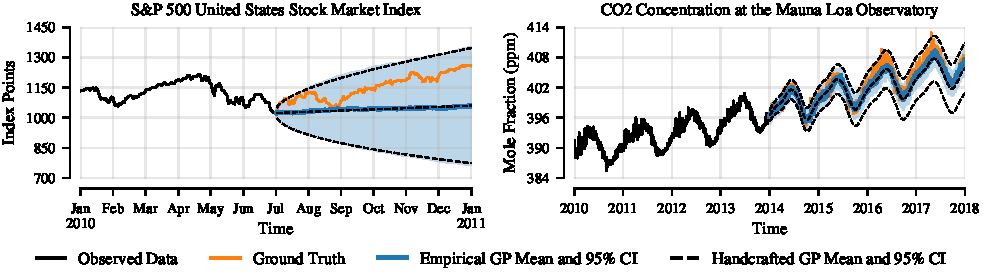
\includegraphics[width=6.4in]{fig/empirical_vs_handcrafted.pdf}
    \caption{
    Without human intervention, Empirical GP captures the behavior of kernels handcrafted by human experts. \textbf{Left:} On financial stock market data, Empirical GP matches the canonical geometric Brownian motion model. While it cannot be expected to predict future prices exactly, it recovers the optimal statistical variance and drift of the data-generating process.
    \textbf{Right:} On atmospheric climate data, Empirical GP infers seasonality and an upwards trend, achieving 21\% lower RMSE than an expert-designed kernel~\cite{rasmussen2024co2model}.
    }
    \label{fig:empirical_vs_handcrafted}
\end{figure*}

%%%%%%%%%%%%%%%%%%%%%%%%%%%%%%%%%%%%%%%%%%%%%%%%%%%%%%%%%%%%%%%%%%%%%%%%%%%%%%
\section{Introduction}
\label{sec:introduction}
Gaussian processes (GPs) provide an elegant framework for probabilistic regression, offering data efficiency and principled uncertainty quantification essential for applications ranging from scientific modeling to Bayesian optimization \citep{rasmussen2006gaussian}.
However, the practical utility of GPs hinges on the choice of kernel function, which encodes prior beliefs about the function being modeled.
The kernel function is typically selected from a small set of standard stationary kernels such as radial basis functions (RBF), Mat\'ern, or periodic kernels, and the kernel hyperparameters are estimated by maximizing the marginal log-likelihood.

This approach is limited in its flexibility, since no single kernel is appropriate across all settings. Having an expert hand-craft an artisan kernel can substantially improve the model, but is only feasible for the most critical applications.
\citet{duvenaud2013kernelsearch}  % https://arxiv.org/pdf/1302.4922
and others have tried to overcome this by automatically constructing kernel compositions in a data-driven fashion,
but this is still limited to sums and products of canonical kernels, and requires approximations to intractable integrals.  % over kernel hyper-parameters
% but this idea is complex, faces scalability challenges, and is thus not widely adopted in practice.
Finally, many standard kernels are stationary, which
% faces a fundamental limitation when predictions are required beyond the observed data range.
% Stationary kernels assume that the covariance between function values depends only on the distance between inputs, not their absolute locations.
% As a consequence, GP posterior predictions revert to the prior mean in regions far from training data, with uncertainty growing to match the prior variance.
% This behavior
% well-suited for interpolation but
are poorly suited for extrapolation, i.e. predictions at inputs beyond the training range.
The extrapolation problem is common to numerous practical settings, such as predicting the final performance of a machine learning model after observing only the first few epochs of training~\citep{swersky2014freeze, lin2025lkgp}.
Learning curves typically exhibit a characteristic structure of rapid initial improvement followed by gradual saturation, which is consistent across experiments but not captured by stationary kernels.
Similar challenges arise in time series forecasting, where future predictions must extrapolate temporal patterns, and in sequential experimental design, where expensive evaluations must be guided by predictions at unexplored configurations outside the support of the experimental data.

%% [MAX]: Are there non-BO references that could be considered here?
Recent work used historical data to construct more informative GP priors.
\citet{perrone2018scalable,wistuba2021few} consider using neural networks as feature extractors or deep kernels for knowledge transfer in Bayesian optimization. \citet{wang2024hyperbo} proposed pre-training neural networks to parameterize mean and covariance functions for GPs using historical HPO (hyperparameter optimization) datasets. These approaches require careful architecture design, large training corpora to avoid overfitting, and can require time-consuming hyperparameter optimization.

In this paper, we study \emph{Empirical Gaussian Processes}, a framework that takes a fundamentally different approach.
Rather than learning hyperparameters of a parametric kernel, we estimate the GP prior mean and covariance functions directly from a corpus of historical observations of the data-generating stochastic process.
% Our key insight is that when multiple independent realizations of a process are available, e.g. learning curves from previous experiments or trajectories from repeated simulations, we can treat these as samples from the unknown prior and estimate it empirically.
The premise of this approach is that available independent realizations, e.g., learning curves from previous experiments, serve as samples from the unknown prior. %, thereby enabling its empirical estimation.
The empirical prior, properly estimated, will therefore capture structure present in the historical data,
including non-stationarity, heteroscedasticity, and domain-specific correlations.
Unlike parametric kernels that impose rigid assumptions, the empirical covariance adapts to the data, enabling extrapolation that adheres to patterns observed in previous realizations of the process.

Our work revisits the Hierarchical Bayesian framework
of \citet{schwaighofer2004learningGPkernels},
which we extend by generalizing the training algorithm to support spatially heterogeneous observations without grid alignment, and by introducing a novel inference scheme that prevents  overconfidence when extrapolating away from historical data.
% and by providing a rigorous theoretical justification for the continuous limit.
% Empirically, we demonstrate that this efficient approach is competitive with complex, resource-intensive deep learning baselines. We facilitate its adoption by releasing a modern, high-performance PyTorch implementation.

% \claude{Empirical GPs thus offer a unique combination: the meta-learning capability of modern approaches, the convergence guarantees of classical statistics, and the computational simplicity of sample-based estimation. While neural network-based methods require gradient optimization over millions of parameters, we show that sample statistics computed from historical data---the simplest possible estimators---provably converge to the optimal Gaussian prior.}

% We formulate the problem of learning the GP prior from independent datasets as maximum likelihood estimation. Each dataset provides noisy observations of one realization of the underlying process, potentially at different input locations. We derive an Expectation-Maximization (EM) algorithm that iteratively refines estimates of the prior mean and covariance with closed-form updates, enabling efficient computation without Monte Carlo sampling while maintaining exact gradients for optional hyperparameter optimization.

% A particularly elegant special case arises when all datasets contain observations at the same input locations—a common scenario in applications such as learning curve prediction, where models are typically evaluated at fixed training checkpoints. In this matched-observation setting, the EM algorithm converges in a single iteration to the sample mean and sample covariance computed across the historical trajectories. The resulting empirical prior can then be evaluated at arbitrary input locations via interpolation, requiring no iterative optimization whatsoever.

Our main contributions are as follows:
\begin{enumerate}[leftmargin=14pt, labelwidth=!, labelindent=0pt, itemsep=0.8pt]
    \item We introduce Empirical GPs, a principled Bayesian model for learning non-parametric GP priors from independent datasets via maximum likelihood estimation.
    \item We provide function-space-theoretical justification, proving that Empirical GPs converge to the best Gaussian approximation of the true data-generating process.
    \item We derive a closed-form Expectation-Maximization algorithm with exact E- and M-steps, extending prior work from the discrete, fixed-grid setting to continuous domains with sparse, irregularly distributed observations.
    \item We develop a technique to extend the learned prior to new inputs, analogous to inducing point methods but operating directly on the prior to avoid variance starvation.
    \item We demonstrate competitive predictive performance on time series forecasting,
    % (using our dense/interpolated variant)
    learning curve extrapolation,
    and ML hyper-parameter modeling problems,
    % (using our continuous-domain EM variant),
    outperforming multiple optimization-heavy baselines.
\end{enumerate}


%%%%%%%%%%%%%%%%%%%%%%%%%%%%%%%%%%%%%%%%%%%%%%%%%%%%%%%%%%%%%%%%%%%%%%%%%%%%%%
\begin{figure*}[ht]
    \centering
    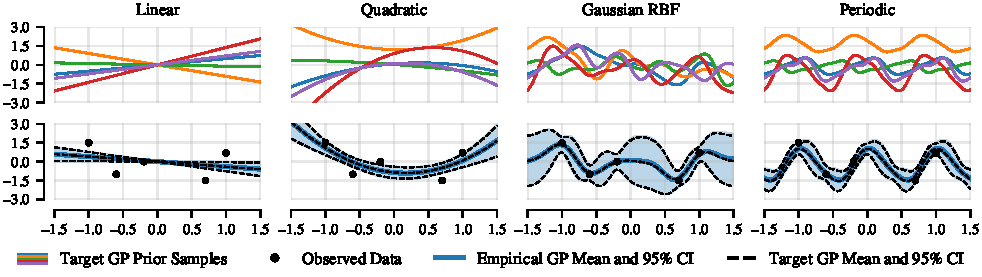
\includegraphics[width=6.75in]{fig/target_gp.pdf}
    \caption{\textbf{Top:} Sample paths from a variety of target GPs with distinct covariances functions are used as historical data for Empirical GP. \textbf{Bottom:} On a fixed set of new observations, the Empirical GP posterior converges to the posterior of the corresponding target GP, when using 256 sample paths from the latter as historical data, demonstrating data-driven adaptivity and convergence to the target GP.}
    \label{fig:target_gp}
\end{figure*}

%%%%%%%%%%%%%%%%%%%%%%%%%%%%%%%%%%%%%%%%%%%%%%%%%%%%%%%%%%%%%%%%%%%%%%%%%%%%%%
\section{Related Work}
\label{sec:related_work}
{\bf Meta-Learning for Gaussian Processes.}
Several approaches learn GP priors from multi-task data.
\citet{zhou2019adaptive} learn basis functions for Bayesian linear regression,
while~\citet{rothfuss2021pacoh} provide PAC-Bayesian guarantees for meta-learning GP hyperparameters.
These methods optimize within parametric kernel families.
In contrast, we follow the idea of~\citet{schwaighofer2004learningGPkernels} and directly estimate the prior mean and covariance functions from sample statistics, yielding a non-parametric prior.

{\bf Multi-Task GPs.}
Multi-task GP methods model correlations between tasks through task kernels \citep{bonilla2007multi, swersky2013multi}, but scale poorly with the number of tasks.
Transfer learning approaches~\citep{salinas2020quantile, feurer2018scalable} offer improved scalability but sacrifice principled uncertainty quantification.

{\bf Variational Inference.}
Our formulation shares similarities with variational GP methods \citep{titsias2009variational, hensman2013gaussian}: both work with finite-dimensional marginals.
However, variational methods approximate a posterior given a fixed prior, whereas we estimate the prior itself.

{\bf Expressive Kernels.}
Deep kernel learning \citep{wilson2016deep} learns flexible features but requires substantial amounts of data and model fitting can suffer from instabilities.
Spectral mixture kernels~\citep{wilson2013gaussian} can extrapolate quasi-periodic patterns but assume stationarity.
Our empirical approach sidesteps these choices: the covariance is estimated directly from data, inheriting whatever structure exists in historical observations.

{\bf Learning Curve Prediction.}
\citet{domhan2015speeding} extrapolate learning curves using parametric models, while \citet{swersky2014freeze} use a GP with a custom exponential mixture kernel to extrapolate learning curves.
\citet{lin2025lkgp} leverage latent Kronecker structure to scalably and jointly model hyper-parameter and learning curve progression dimensions.
\citet{adriaensen2023efficient} train Prior-Fitted Networks (PFNs) on learning curve data sampled from parametric priors.


%%%%%%%%%%%%%%%%%%%%%%%%%%%%%%%%%%%%%%%%%%%%%%%%%%%%%%%%%%%%%%%%%%%%%%%%%%%%%%

\section{Empirical Gaussian Processes}
\label{sec:egps}

\subsection{Preliminaries}
\label{sec:prelim}
A Gaussian Process (GP) is a distribution over functions~$\actualgp$, any finite marginal of which has a joint multivariate normal distribution.
A GP is fully specified by its mean function $m(\mathbf{x}) = \mathbb{E}[\actualgp(\mathbf{x})]$ and its covariance function (kernel) $k(\mathbf{x}, \mathbf{x}') = \mathbb{E}[(\actualgp(\mathbf{x}) - m(\mathbf{x}))(\actualgp(\mathbf{x}') - m(\mathbf{x}'))]$. We write:
\begin{equation}
    \nonumber
    \actualgp(\mathbf{x}) \sim \mathcal{GP}\left(m(\mathbf{x}), k(\mathbf{x}, \mathbf{x}')\right).
\end{equation}
Any valid kernel function must be positive semi-definite (PSD). That is, for any set of input points $\{\mathbf{x}_1, \ldots, \mathbf{x}_N\} \subset \domain$ and any non-zero vector $\mathbf{v} \in \mathbb{R}^N$, the kernel matrix $\mathbf{K}$ with entries $K_{ij} = k(\mathbf{x}_i, \mathbf{x}_j)$ must satisfy $\mathbf{v}^\top \mathbf{K} \mathbf{v} \geq 0$.

\subsection{Function-Space View}
\label{subsec:egps:general}
Suppose we want to approximate a data-generating stochastic process.
Given $\K$ independent sample paths $f_1, \ldots, f_\K$,
we can estimate their true mean $m = \mathbb{E}[f]$ and covariance function $k = \mathrm{Cov}(f)$ via maximum likelihood,
\begin{equation}
\label{eq:empirical_mean_and_kernel}
   \begin{aligned}
        m_\K(\mathbf{x}) = \frac{1}{\K} \sum_{i=1}^{\K} f_i(\mathbf{x}), \ \
        k_\K(\mathbf{x}, \mathbf{x}') = \frac{1}{\K} \sum_{i=1}^{\K}
         \tilde \sample_i(\vx) \tilde \sample_i(\vx'),
    \end{aligned}
\end{equation}
where $\tilde \sample_i(\vx) = f_i(\vx) - m(\vx)$.
We define the \emph{Empirical} GP using the \emph{empirical} mean $m_S$ and covariance function $k_S$ as $\mathcal{GP}\bigl(m_\K, k_\K\bigr)$.
Note that $k_\K$ is a valid kernel by construction, as it is a sum of outer products of the centered functions.

\subsection{Theoretical Results}
\label{subsec:egp:theory}

We now provide a selection of key theoretical results that ground our approach.
A more formal treatment including all assumptions and proofs is given in Appendix~\ref{apd:theory}.

Let $\mathcal{GP}\bigl(m_\K, k_\K\bigr)$ be the Empirical GP defined by the empirical mean function $m_\K$ and empirical covariance function $k_\K$, conditioned on observed sample paths $f_1, ..., f_\K$.
Additionally, let $\mathcal{GP}\bigl(m, k)$ be a GP defined by the true mean function $m$ and true covariance function $k$ of $\stochprocess$.
%%%%%%%%
\begin{restatable}{proposition}{WeakConvergence}
\label{thm:weak_convergence}
Assume that $k$ is continuous and that its canonical semi-metric satisfies Dudley's entropy integral condition.
Then, for almost every sequence of sample paths $\{ f_i \}_{i=1}^\K$, we have $\mathcal{GP}\bigl(m_\K, k_\K\bigr) \rightharpoonup \mathcal{GP}\bigl(m, k)$ as $\K \to \infty$.
\end{restatable}
In particular, the limit $\mathcal{GP}\bigl(m, k)$ is the best possible Gaussian approximation of the true underlying stochastic process in terms of the KL divergence definition by \citet{sun2019functional}.
\begin{restatable}{proposition}{KLD}
\label{thm:kl_divergence}
Let $\mathbb{P}$ denote the law of $f$, and let $\mathbb{G}$ be any GP indexed by $\domain$.
Assume that $\mathbb{P}$ is absolutely continuous with respect to $\mathbb{G}$, and that $k$ is strictly positive definite.
Then,
$\lim_{\K \to \infty} \mathcal{GP}\bigl(m_\K, k_\K\bigr) = \arg\! \min_\mathbb{G} \; D_{\mathrm{KL}} ( \mathbb{P} \;\Vert\; \mathbb{G})$.
\end{restatable}

\Cref{{thm:kl_divergence}} provides firm theoretical grounding for the use of Empirical GPs as a general modeling approach for learning from historical data.

\begin{figure*}[ht]
    \centering
    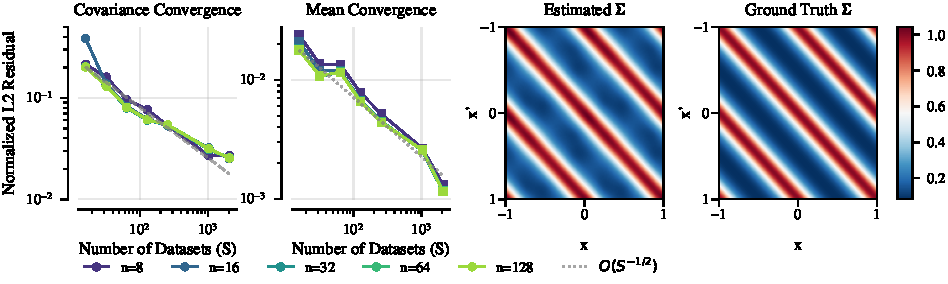
\includegraphics[width=6.75in]{fig/em_convergence_discrete_case.pdf}
    \caption{
    \textbf{Left:} Convergence of the EM-estimated prior mean and covariance to the ground truth, as a function of the number of independent incomplete datasets (\K), and for different numbers of observed data points per dataset (n).
    \textbf{Right:} The estimated covariance matrix ($\K = 1024, n = 64$) follows the ground truth closely.}
    \label{fig:em_convergence_discrete_case}
    \vspace{-1ex}
\end{figure*}

% \subsection{Discrete Observations}
% In practice, we cannot observe full continuous sample paths, nor do we always observe the process at a fixed set of aligned coordinate locations. Real-world data arrives as finite, discrete sets of observations $\{\mathbf{X}_i, \mathbf{y}_i\}$, where the input locations $\mathbf{X}_i$ may vary arbitrarily from sample to sample.

% % \paragraph{Densely sampled and low-dimensional settings}
% % -- such as high-frequency time series --
% % one can approximate the continuous statistics by defining the empirical mean and covariance functions using interpolants of the raw data.

% Important special cases are {\it densely sampled and low-dimensional settings}
% -- such as high-frequency time series --
% where we can approximate continuous statistics by defining empirical mean and covariance functions via interpolants of the raw data.
% This approach essentially treats the interpolated paths as fully observed functions,
% allowing for the direct computation of empirical statistics in Eq.~\ref{eq:empirical_mean_and_kernel}.
% Despite its simplicity, this heuristic often leads to surprisingly strong results,
% see our experimental results in Sec.~\ref{sec:gift_eval_experiments},
% where such a linear-interpolation-based Empirical GP
% outperforms several deep learning models on time series forecasting.

% {\color{red} TODO: Talk about SVD acceleration briefly, but point reader to the appendix for details}

\subsection{Discrete Observations}
\label{sec:discrete_observations}
In practice, we cannot observe full continuous sample paths. Real-world data arrives as finite, discrete sets of observations $\{\mathbf{X}_i, \mathbf{y}_i\}$, where the input locations $\mathbf{X}_i$ may vary arbitrarily from sample to sample.

Important special cases are \textit{densely sampled and low-dimensional settings}—such as high-frequency time series—where we can approximate the continuous statistics via interpolation. Formally, for each sample $i$, we define an (e.g. linear) interpolant $\tilde{f}_i(\cdot) = \mathcal{I}(\cdot; \mathbf{X}_i, \mathbf{y}_i)$, and
treat $\tilde{f}_i$ as fully observed realizations of the process, allowing us to evaluate the empirical covariance in~\eqref{eq:empirical_mean_and_kernel} directly at \textit{arbitrary} input locations.
% \begin{equation}
% \nonumber
%     \label{eq:interp_covariance}
%     \hat k(x, x') \approx \frac{1}{\K} \sum_{i=1}^\K (\tilde{f}_i(x) - \hat{m}(x))(\tilde{f}_i(x') - \hat{m}(x')).
% \end{equation}
Despite its simplicity, this heuristic leads to surprisingly strong results; as shown in Sec.~\ref{sec:gift_eval_experiments}, this interpolation-based Empirical GP outperforms several deep learning models on a time series forecasting benchmark.

\paragraph{Efficient Computation via SVD}
While evaluating~\eqref{eq:empirical_mean_and_kernel} is efficient, the cost scales linearly with the number of historical samples $\K$. To further accelerate inference for large datasets, we discretize the interpolants onto a shared reference grid
$\mathbf{Z} = \{\mathbf{z}_1, \cdots, \mathbf{z}_M\}$
to form a matrix $\mathbf{Y} \in \mathbb{R}^{\K \times M}$ of centered observations. We then employ a lossless compression using an SVD,
$\mathbf{Y} = \mathbf{U} \mathbf{S} \mathbf{V}^\top$,
constructing a reduced set of $M$ ``eigen-observations'' $\tilde{\mathbf{Y}} = \mathbf{S}\mathbf{V}^\top \in \mathbb{R}^{M \times M}$.
Interpolating the scaled eigen-observations $\tilde{v}_j(\cdot) = \mathcal{I}(\cdot; \mathbf{Z}, [\tilde{\mathbf{Y}}]_j)$ enables kernel evaluation at arbitrary locations while reducing complexity from $\mathcal{O}(\K)$ to $\mathcal{O}(M)$ by replacing the full dataset with $M$ basis functions.

%%%%%%%%%%%%%%%%%%%%%%%%%%%%%%%%%%%%%%%
\subsection{Continuous-Domain Empirical Gaussian Process}
\label{subsec:egps:em}

We now address the more general and challenging scenario where observations are sparse and irregularly distributed. In these regimes, geometric interpolation is ill-defined, and sample statistics cannot be computed directly.
Instead, we employ a kernel-based mechanism to probabilistically project sparse data onto shared latent variables. This establishes a rigorous generative model that couples the disparate observation sets $\mathbf{X}_i$ through a unified latent structure.

To formalize this framework, we anchor the latent process on a fixed set of $M$ reference locations $\mathbf{Z} = \{\mathbf{z}_1, \ldots, \mathbf{z}_M\} \subset \mathcal{X}$.
We treat the corresponding function values $\mathbf{u} = f(\mathbf{Z}) \in \mathbb{R}^M$ as the latent variables.
For each historical sample $i$, we observe a vector $\mathbf{y}_i$ at a unique set of input locations $\mathbf{X}_i$ of size $N_i$. Our goal is to recover the population parameters $\boldsymbol{\mu}$ and $\boldsymbol{\Sigma}$ of the latent variables $\mathbf{u}$ that best explain the observations $\{\mathbf{X}_i, \mathbf{y}_i\}_{i=1}^{\K}$.

\paragraph{Interpolation Mechanism}
To relate the latent variables $\mathbf{u}$ at $\mathbf{Z}$ to observations at arbitrary locations $\mathbf{X}_i$, we use kernel interpolation based on a stationary base kernel $k_{\text{base}}(\cdot, \cdot)$. We define the weight matrix $\mathbf{W}_i \in \mathbb{R}^{N_i \times M}$ as
$\mathbf{W}_i~=~k_{\text{base}}(\mathbf{X}_i, \mathbf{Z}) \, k_{\text{base}}(\mathbf{Z}, \mathbf{Z})^{-1}$.

\paragraph{Probabilistic Model}
We assume the latent reference values $\mathbf{u}_i$ for each task are drawn from a shared multivariate normal prior:
\begin{equation}
\nonumber
    \mathbf{u}_i \sim \mathcal{N}(\boldsymbol{\mu}, \boldsymbol{\Sigma}), \quad i = 1, \ldots, \K.
\end{equation}

The observations $\mathbf{y}_i$ are modeled as the projected latent values with additive Gaussian noise:
\begin{equation}
\nonumber
    \mathbf{y}_i \mid \mathbf{u}_i \sim \mathcal{N}(\mathbf{W}_i \mathbf{u}_i, \sigma^2 \mathbf{I}),
\end{equation}
where $\sigma^2$ is the variance of the measurement noise.
% This formulation treats the function values between reference points as deterministically interpolated, simplifying the inference while allowing for spatially distinct observation sets.
This formulation decouples the shared latent structure on $\mathbf{Z}$ from the task-specific observation locations $\mathbf{X}_i$, allowing us to aggregate information from spatially heterogeneous datasets.

\paragraph{E-step (Imputation)}
We compute the posterior distribution of the latent variables $\mathbf{u}_i$ given the partial observations $\mathbf{y}_i$ and current parameter estimates $\boldsymbol{\mu}^{(t)}, \boldsymbol{\Sigma}^{(t)}$. This posterior is Gaussian:
\begin{equation}
\nonumber
    p(\mathbf{u}_i \mid \mathbf{y}_i) = \mathcal{N}(\mathbf{m}_i, \mathbf{C}_i).
\end{equation}
To streamline the notation, we define the \textit{cross-covariance} between the reference grid and the observation locations as $\bSigma_{\bZ, \bX_i} = \boldsymbol{\Sigma}^{(t)} \mathbf{W}_i^\top$. The moments are computed as:
\begin{equation}
\nonumber
    \begin{aligned}
            \mathbf{m}_i &= \boldsymbol{\mu}^{(t)} + \boldsymbol{\Sigma}_{\bZ, \bX_i}  \bSigma_{\bX_i, \bX_i} ^{-1} \left(
                \mathbf{y}_i - \mathbf{W}_i \boldsymbol{\mu}^{(t)}
            \right), \\
    \mathbf{C}_i &= \boldsymbol{\Sigma}^{(t)} - \boldsymbol{\Sigma}_{\bZ, \bX_i} \bSigma_{\bX_i, \bX_i}^{-1} \boldsymbol{\Sigma}_{\bX_i, \bZ},
    \end{aligned}
\end{equation}
where $\bSigma_{\bX_i, \bX_i}  = \mathbf{W}_i \bSigma \mathbf{W}_i^\top + \sigma^2 \mathbf{I}$ is the predicted covariance at the observed locations. This highlights that the update is a standard correction term weighted by the correlation between the latent grid and the specific observations.

% Here, $\boldsymbol{\Sigma}_{\cdot, \IndexSet_i}^{(t)}$ denotes the columns of the covariance matrix corresponding to the observed indices, effectively mapping information from observed locations to the entirety of $\bX$.

\paragraph{M-step (Maximum Likelihood)}
We update the parameters by maximizing the expected log-likelihood. The updates simply aggregate the sufficient statistics from all tasks:
\begin{equation}
\nonumber
    \begin{aligned}
        \boldsymbol{\mu}^{(t+1)} = \frac{1}{\K} \sum_{i=1}^{\K} \mathbf{m}_i, \qquad
        \boldsymbol{\Sigma}^{(t+1)} = \frac{1}{\K} \sum_{i=1}^{\K} \mathbf{C}_i + \mathbf{\tilde m}_i \mathbf{\tilde m}_i^{\!\top},
\end{aligned}
\end{equation}
where $\mathbf{\tilde m}_i = \mathbf{m}_i - \boldsymbol{\mu}^{(t+1)}$.

\paragraph{Extensions}
Shrinking the rank-deficient M-step toward a structured target is exactly MAP-EM under an Inverse-Wishart prior (\Cref{apd:shrinkage}); a fitted base kernel can augment the prior at conditioning time (\Cref{apd:base_augmented}); and the estimator extends to multi-output and multi-task settings (\Cref{apd:multioutput,apd:multitask}).

\paragraph{Computational Complexity}
The computational cost of the EM iterations is determined by the size of the reference set $M$ and the per-task observation count $N_i$.
Computing the interpolation weights $\mathbf{W}_i$ requires $\mathcal{O}(N_i M^2)$.
In the E-step, forming the predictive covariance $\boldsymbol{\Sigma}_{\bX_i, \bX_i}$ and inverting it requires $\mathcal{O}(N_i M^2 + N_i^3)$ operations.
The M-step is dominated by the summation of the conditional covariances $\mathbf{C}_i$, which is $\mathcal{O}(\K M^2)$.
Thus, the algorithm's complexity is dominated by the E-step $\mathcal{O}(\K (N_iM^2 + N_i^3))$. For datasets with large $N_i > M$, one can exploit the Woodbury identity to reduce the inversion cost to $\mathcal{O}(M^3 + N_i M^2)$.


%%%%%%%%%%%%%%%%%%%%%%%%%%%%%%%%%%%%%%%
\paragraph{Residual Interpolation and Base Kernel}
The kernel-interpolation described above restricts the learned correlations to a neighborhood of the reference set $\mathbf{Z}$. Consequently, at test locations $\mathbf{X}_*$ far from $\mathbf{Z}$ where the interpolation weights vanish ($\mathbf{W}_* \to \mathbf{0}$), the predictive variance collapses to the noise floor. This leads to exceedingly high confidence in regions where the model should exhibit high epistemic uncertainty, that is, variance starvation.

To resolve this, we employ a residual interpolation scheme.
 Instead of assuming the latent variables $\mathbf{u}$ capture the total function, we interpret the learned parameters $\boldsymbol{\mu}$ and $\boldsymbol{\Sigma}$ on the grid $\mathbf{Z}$ as non-parametric adjustments (``shifts'') to a base parametric mean function $\mu_{\text{base}}(\cdot)$ and kernel $k_{\text{base}}(\cdot, \cdot)$. We define the learned residuals at the reference locations as:
\begin{equation}
\nonumber
    \boldsymbol{\delta}_{\mu} = \boldsymbol{\mu} - \mu_{\text{base}}(\mathbf{Z}), \qquad
    \boldsymbol{\delta}_{\Sigma} = \boldsymbol{\Sigma} - k_{\text{base}}(\mathbf{Z}, \mathbf{Z}).
\end{equation}
These quantities capture the structural, non-stationary deviations that the base model fails to explain.
To generalize to new inputs $\mathbf{x}$, we project these residuals through the base kernel structure:
\begin{equation}
\label{eq:residual_interpolant}
\begin{aligned}
    \mu(\mathbf{x}) &= \mu_{\text{base}}(\mathbf{x}) + \mathbf{W}_{\mathbf{x}} \boldsymbol{\delta}_{\mu}, \\
    k(\mathbf{x}, \mathbf{x}') &= k_{\text{base}}(\mathbf{x}, \mathbf{x}') + \mathbf{W}_{\mathbf{x}} \boldsymbol{\delta}_{\Sigma} \mathbf{W}_{\mathbf{x}'}^\top,
\end{aligned}
\end{equation}
where $\mathbf{W}_{\mathbf{x}} = k_{\text{base}}(\mathbf{x}, \mathbf{Z}) k_{\text{base}}(\mathbf{Z}, \mathbf{Z})^{-1}$.

Therefore, the base kernel $k_{\text{base}}$ does not serve as a rigid assumption or a noise floor.
Instead, this formulation explicitly decouples two complementary types of behaviors:
% \begin{enumerate}
% \item {\it Within-Domain Extrapolation} Within the range of historical support, the Empirical GP uses the learned non-stationary trends and seasonal dynamics to project future sample paths without reverting prematurely to an uninformative prior mean.
% \item {\it Off-Grid Robustness} Far away from any historical coordinates where $\mathbf{W}_{\mathbf{x}} \to \mathbf{0}$, the prior gracefully reverts to the baseline behavior of $k_{\text{base}}$, providing reliable epistemic uncertainty bounds in completely unobserved territory.
% \end{enumerate}

1) {\it Within-Domain Extrapolation:} Within the range of the historical support, Empirical GPs use the learned non-stationary covariances to extrapolate sample paths without reverting prematurely to an uninformative prior mean.

2) {\it Off-Grid Robustness:} Far from any historical coordinates,
where $\mathbf{W}_{\mathbf{x}} \to \mathbf{0}$,
the prior gracefully reverts to the baseline behavior of $k_{\text{base}}$.
While this introduces a dependency on $k_{\text{base}}$,
the base mean and kernel can simple be chosen and optimized as a canonical GP,
and then used for the EM-algorithm above.
This straightforward approach is sufficient to outperform competing methods on
a 7-dimensional hyper-parameter modeling problem in Section~\ref{sec:higher_dim_experiments}.

\paragraph{Residual Interpolation in Training}
Leveraging residual interpretation also requires a modification of the E-step.
Treating the projection
$\mathbf{W}_i\mathbf{u}_i$ as exact ignores the base-kernel variance at
$\mathbf{X}_i$ not captured by $\mathbf{Z}$.
Instead, we set
\begin{equation}
\nonumber
    \mathbf{Q}_i = \big(\mathbf{K}_{\mathbf{X}_i\mathbf{X}_i}
    - \mathbf{W}_i \mathbf{K}_{\mathbf{ZZ}} \mathbf{W}_i^\top\big) + \sigma^2 \mathbf{I},
\end{equation}
so that $\mathbf{y}_i \mid \mathbf{u}_i \sim \mathcal{N}(\mathbf{W}_i\mathbf{u}_i, \mathbf{Q}_i)$.
% Substituting $\mathbf{Q}_i$ for $\sigma^2\mathbf{I}$ in
% $\boldsymbol{\Sigma}_{\mathbf{X}_i,\mathbf{X}_i}$ raises the E-step inversion to
% $\mathcal{O}(N_i^3)$ but is what makes the variance-starvation fix consistent
% during training on sparse, irregular data.

\paragraph{Relation to Inducing Points}
Equation~\eqref{eq:residual_interpolant} has similarities to variational
inducing-point methods \citep{titsias2009variational}, but with a crucial
difference: we use it to \emph{define the prior}, whereas variational methods
use an analogous expression to \emph{approximate the posterior} under a fixed
prior. Consequently, the variational posterior mean is confined to a rank-$M$
subspace, while the posterior mean induced by the Empirical GP prior can occupy an
arbitrarily high-rank space with an appropriate base kernel.

% \paragraph{Modifications to the EM Algorithm}
% During training, this residual interpretation manifests as a structured noise model. For a historical task observed at $\mathbf{X}_i$, the conditional distribution of the observations becomes:
% \begin{equation}
% \nonumber
%     \mathbf{y}_i \mid \mathbf{u}_i \sim \mathcal{N}(\mathbf{W}_i \mathbf{u}_i, \mathbf{Q}_i).
% \end{equation}
% The effective noise covariance $\mathbf{Q}_i$ now accounts for the residual variance of the base kernel that is orthogonal to the reference set:
% \begin{equation}
% \nonumber
%     \mathbf{Q}_i = \underbrace{(\mathbf{K}_{\mathbf{X}_i \mathbf{X}_i} - \mathbf{W}_i \mathbf{K}_{\mathbf{ZZ}} \mathbf{W}_i^\top)}_{\text{Interpolation Uncertainty}} + \sigma^2 \mathbf{I}.
% \end{equation}
% To implement Residual-Interpolation, we simply replace the diagonal noise $\sigma^2 \mathbf{I}$ with the dense matrix $\mathbf{Q}_i$ when computing the marginal covariance $\boldsymbol{\Sigma}_{\bX_i, \bX_i}$ in the E-step. While this increases the computational cost of the inversion to $\mathcal{O}(N_i^3)$, it provides the necessary robustness for learning from sparse, irregular data.

\begin{figure*}[ht!]
    \centering
    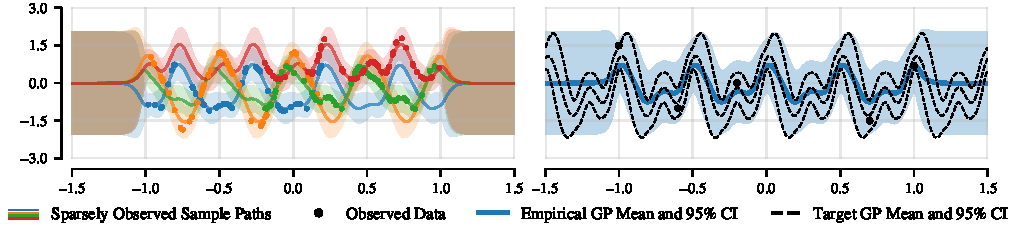
\includegraphics[width=6.75in]{fig/em_gp_interp.pdf}
    \caption{
    \textbf{Left:} The EM-inferred conditional distributions
    for each set of independent historical observations (points).
    The historical inputs are sampled uniformly from one of two continuous intervals: (-1, 0.2) and (-0.2, 1). The EM-inferred conditional distributions exhibit the periodic characteristics beyond the respective interval associated with a given set of historical observations, and revert gracefully to the base kernel (Matérn) beyond the range of any historical observations (-1, 1).
    \textbf{Right:} The posterior distribution associated with the EM-inferred GP prior (blue), compared to the ground truth posterior (dashed). The Empirical GP closely follows the ground truth within the interval of historical observations (-1, 1), and reverts back to the base kernel's behavior beyond.
    }
    \label{fig:em_gp_interp}
    \vspace{-1ex}
\end{figure*}

% \paragraph{Computational Complexity.}
% The complexity of the EM iterations depends on the ratio of
% observed elements per sample $\rho = \max_i |\IndexSet_i| / N$.
% The Cholesky decompositions in the E-step
% require $\mathcal{O}(\K (N \rho)^3)$ operations,
% and the formation of the conditional covariances $\mathbf{C}_i$
% require an additional $\mathcal{O}(\K N^2 \rho)$.
% The M-step is dominated by the summation of the conditional covariances,
% which is $\mathcal{O}(\K N^2)$.
% Therefore, the overall complexity if $\mathcal{O}(\K N^2 (1 + N \rho^3))$.
% The observed convergence speed of the algorithm increases as on the missingness ratio decreases,
% and reduces to the computation of the sample mean and covariance in the case of
% fully observed noiseless samples.
% See also Sec.~\ref{sec:em_convergence_speed}
% for a study on the convergence speed
% as a function of $\rho$.

% \paragraph{Extension to Continuous Inputs}

% The EM algorithm described above estimates the prior parameters $\boldsymbol{\mu} \in \mathbb{R}^N$ and $\boldsymbol{\Sigma} \in \mathbb{R}^{N \times N}$ exclusively on the fixed grid of historical locations $\mathbf{Z}$.
% To extend this learned prior for predictions at new input locations $\mathbf{X}_*$, we employ a interpolation scheme
% that interprets the learned grid parameters as non-parametric adjustments to a base parametric mean function $m(\cdot)$ and kernel function $k(\cdot, \cdot)$.
% We define the learned residuals (``shifts'') at the reference locations $\mathbf{X}$ as:
% \begin{equation}
% \nonumber
%     \begin{aligned}
%         \boldsymbol{\delta}_{\mu} &= \boldsymbol{\mu} - m(\mathbf{X}), \qquad
%         \boldsymbol{\delta}_{\Sigma} &= \boldsymbol{\Sigma} - k(\mathbf{X}, \mathbf{X}).
%     \end{aligned}
% \end{equation}

% These quantities capture the structure in the data that the base parametric model fails to explain. To generalize to new inputs, we project these shifts through the base kernel structure. The interpolated mean and covariance at $\mathbf{X}_*$ are given by:
% \begin{equation}
% \label{eq:shift_interpolant}
% \begin{aligned}
%     \boldsymbol{\mu}(\mathbf{X}_*) &= m(\mathbf{X}_*) + \mathbf{W} \boldsymbol{\delta}_{\mu}, \\
%     \boldsymbol{\Sigma}(\mathbf{X}_*, \mathbf{X}_*) &= k(\mathbf{X}_*, \mathbf{X}_*) + \mathbf{W} \boldsymbol{\delta}_{\Sigma} \mathbf{W}^\top,
% \end{aligned}
% \end{equation}
% where $\mathbf{W} = \mathbf{K}_{*X} \mathbf{K}_{XX}^{-1}$ is the matrix of kernel weights, and $\mathbf{K}_{*X} = k(\mathbf{X}_*, \mathbf{X})$.
% Note that this kernel inherits the positive (semi-)definite properties of the base kernel $k$, see Lemma~\ref{lem:shift_interapolant_psd}.

% This formulation has two key properties. First, it ensures exact consistency: if $\mathbf{X}_* = \mathbf{Z}$, the interpolated moments exactly recover the EM estimates $\boldsymbol{\mu}$ and $\boldsymbol{\Sigma}$. Second, it provides a smooth extrapolation of the learned correlation structure to off-grid points, reverting to the base kernel behavior far from the historical data $\mathbf{X}$ if $k$ is stationary. {\color{red} Shall we prove this, and make a Lemma that summarizes all the properties, including PSD?}


%%%%%%%%%%%%%%%%%%%%%%%%%%%%%%%%%%%%%%%% INDUCING POINT VERSION %%%%%%%%%%%
% \subsection{Probabilistic Model \& Inducing Points}

% To scale the estimation to many historical data points, we introduce a set of fixed inducing locations $\mathbf{Z} = \{\mathbf{z}_1, \ldots, \mathbf{z}_M\}$. While this mimics the inducing point approach that is well-known from sparse GPs \citep{snelson2005sparse}, we emphasize that in our setting is the \emph{prior} that we approximate in this way, rather than the posterior.

% We define the global parameters as the mean vector $\boldsymbol{\mu} \in \mathbb{R}^M$ and covariance matrix $\boldsymbol{\Sigma} \in \mathbb{R}^{M \times M}$ evaluated at these locations.
% The latent function values $\samplevec_Z$ at the inducing locations are shared across data sets:
% \begin{equation}
%     \samplevec_Z \sim \mathcal{N}(\boldsymbol{\mu}, \boldsymbol{\Sigma}).
% \end{equation}
% For a specific data set $i$ with inputs $X_i$, we assume the latent values $\samplevec_{X_i}$ are derived from $\samplevec_Z$ via a \textit{shift-based interpolation}. This interprets the learned parameters as perturbations of a base parametric mean $m(\cdot)$ and kernel $k(\cdot, \cdot)$:
% \begin{align}
%     \boldsymbol{\mu}_{X_i} &= m(X_i) + \mathbf{W}_i (\boldsymbol{\mu} - m(\mathbf{Z})), \\
%     \boldsymbol{\Sigma}_{X_i X_i} &= \mathbf{K}_{X_i X_i} + \mathbf{W}_i (\boldsymbol{\Sigma} - k(\mathbf{Z}, \mathbf{Z})) \mathbf{W}_i^\top,
% \end{align}
% where $\mathbf{W}_i = \mathbf{K}_{X_i Z} \mathbf{K}_{ZZ}^{-1}$. The observations follow $\mathbf{y}_i \mid \samplevec_Z \sim \mathcal{N}(\boldsymbol{\mu}_{X_i} + \mathbf{W}_i(\samplevec_Z - \boldsymbol{\mu}), \sigma^2 \mathbf{I})$.
% One important characteristic of this interpolation method is that
% we recover the estimated covariance $\boldsymbol{\Sigma}$ when evaluating the kernel on the inducing locations (which could be equal to the union of historical points),
% and revert back to the base kernel $k$ in a controlled fashion, when evaluating far away from any historically observed input.
% This ensures that the model reverts gracefully to the behavior of
% a canonical GP in parts of the space where no informative empirical data exists.

% \subsection{EM Algorithm}

% We estimate $\samplevec = \{\boldsymbol{\mu}, \boldsymbol{\Sigma}\}$ using the Expectation-Maximization (EM) algorithm.

% \paragraph{E-step.}
% We compute the posterior distribution of the inducing variables $p(\samplevec_Z \mid \mathbf{y}_i) = \mathcal{N}(\mathbf{m}_i,  \mathbf{C}_i)$ given the current estimates $\boldsymbol{\mu}^{(t)}, \boldsymbol{\Sigma}^{(t)}$, where $\mathbf{m}_i$ is the posterior mean of inducing points for dataset $i$. The sufficient statistics are:
% \begin{align}
%     \mathbf{m}_i &= \boldsymbol{\mu}^{(t)} + \boldsymbol{\Sigma}_{Z X_i}^{(t)} \mathbf{\Lambda}_i^{-1} \Bigl(\mathbf{y}_i - \boldsymbol{\mu}_{X_i}^{(t)}\Bigr), \\
%     \mathbf{C}_i &= \boldsymbol{\Sigma}^{(t)} - \boldsymbol{\Sigma}_{Z X_i}^{(t)} \mathbf{\Lambda}_i^{-1} \Bigl(\boldsymbol{\Sigma}_{Z X_i}^{(t)}\Bigr)^{\!\top},
% \end{align}
% where $\mathbf{\Lambda}_i = \boldsymbol{\Sigma}_{X_i X_i}^{(t)} + \sigma^2 \mathbf{I}_{n_i}$ is the marginal likelihood covariance for data set $i$, and $\boldsymbol{\Sigma}_{Z X_i}$ is the cross-covariance derived from the shift interpolation.

% \paragraph{M-step (Maximum Likelihood).}
% We update the parameters by maximizing the expected log-likelihood. The updates aggregate the posterior moments from all $K$ tasks:
% \begin{align}
%     \boldsymbol{\mu}^{(t+1)} &= \frac{1}{\K} \sum_{i=1}^{K} \mathbf{m}_i, \label{eq:mu_ml} \\
%     \boldsymbol{\Sigma}^{(t+1)} &= \frac{1}{\K} \sum_{i=1}^{K} \left[ \mathbf{C}_i + (\mathbf{m}_i - \boldsymbol{\mu}^{(t+1)})(\mathbf{m}_i - \boldsymbol{\mu}^{(t+1)})^\top \right]. \label{eq:sigma_ml}
% \end{align}

%%%%%%%%%%%%%%%%%%%

% \paragraph{Regularization via Inverse-Wishart Prior.}
% In settings with limited data (small $K$), the ML estimation of $\boldsymbol{\Sigma}$ may be unstable or the estimate may be singular. We can regularize the estimation by placing an Inverse-Wishart prior on the covariance: $\boldsymbol{\Sigma} \sim \mathcal{IW}(\boldsymbol{\Psi}, \nu)$.  This modifies the M-step update to:
% \begin{equation}
%     \boldsymbol{\Sigma}_{\text{MAP}}^{(t+1)} = \frac{\boldsymbol{\Psi} + K \boldsymbol{\Sigma}_{\text{ML}}^{(t+1)}}{K + \nu + M + 1}.
% \end{equation}
% This acts as a shrinkage estimator: the empirical covariance is pulled towards the prior structure encoded in $\boldsymbol{\Psi}$ (typically the base kernel matrix), stabilizing the optimization.

% \paragraph{Marginal Log-Likelihood.}
% For hyperparameter optimization, we maximize the sum of marginal log-likelihoods
% over all datasets:
% \begin{equation}
%     \mathcal{L}(\boldsymbol{\phi}) = \sum_{i=1}^{K} \log p(\mathbf{y}_i \mid
%     \boldsymbol{\mu}, \boldsymbol{\Sigma}, \sigma^2),
% \end{equation}
% where $\boldsymbol{\phi}$ denotes the hyperparameters of the initial mean and
% kernel functions. Since the EM updates are differentiable, gradients flow through
% the entire estimation procedure, enabling end-to-end optimization.


%%%%%%%%%%%%%%%%%
\subsection{Related Approaches}
\label{subsec:egps:relations}
\citet{schwaighofer2004learningGPkernels} similarly employ an EM for non-parametric covariance learning, compared to which our approach introduces two critical advancements.
First, \citet{schwaighofer2004learningGPkernels} rely on a fixed-grid discretization, while the probabilistic interpolation mechanism above enables training directly on spatially heterogeneous, continuous observations without alignment.
Second, we address the \textit{variance starvation} inherent in their Nystr\"{o}m-based prediction, where uncertainty collapses to zero away from the reference set, ensuring robust uncertainty quantification that reverts gracefully to the base prior in unexplored regions.

% HyperBO~\citep{wang2024hyperbo} pre-trains a Deep Kernel GP~\citep{wilson2016deep} by minimizing the negative log-marginal likelihood via gradient-based optimization.
% In the simple case of fully observed samples on a shared grid,
% this objective is equivalent to minimizing the KL divergence from the empirical distribution defined by the sample moments~\citep{wang2024hyperbo}.
% Notably, our non-parametric estimator achieves this minimum KL solution by definition,
% recovering the exact empirical statistics, whereas HyperBO approximates this target via a parametric kernel on an MLP embedding.
% Furthermore, the EM algorithm relies on stable, closed-form updates,
% avoiding the extensive iterations and instabilities
% associated with gradient-based methods.

HyperBO~\citep{wang2024hyperbo} optimizes a Deep Kernel GP ($k_{\theta}(\mathbf{x}, \mathbf{x}') = k_{\nu}(\phi_\theta(\mathbf{x}), \phi_\theta(\mathbf{x}'))$) via gradient descent.
While expressive, the learned correlations are implicit within the network weights $\theta$, making the prior difficult to interpret.
In contrast, our EM approach explicitly estimates the covariance matrix $\boldsymbol{\Sigma}$ on reference inputs,
and enables stable, closed-form updates, avoiding the extensive iterations and instabilities of gradient-based methods.

% In the simple case of fully observed samples on a shared grid, this objective is equivalent to minimizing the KL divergence from the empirical distribution defined by the sample moments~\citep{wang2024hyperbo}.
% Notably, our non-parametric estimator achieves this minimum KL solution by definition, recovering the exact empirical statistics, whereas HyperBO is restricted to the approximation capacity of the deep kernel.

% Another prominent approach, HyperBO~\citep{wang2024hyperbo}, pre-trains a Deep Kernel GP~\citet{wilson2016deep}
% by minimizing the negative log-marginal likelihood via gradient descent.
% The theoretical relationship between our methods is best understood in the idealized limit of fully observed samples $\sample_i(\bX)$ on a shared grid $\bX$ (the ``matching-input'' setting).
% In this regime, minimizing the log-likelihood is equivalent to minimizing the Kullback-Leibler divergence from the empirical distribution defined by the sample moments $(\hat{\boldsymbol{\mu}}, \hat{\boldsymbol{\Sigma}})$~\citep{wang2024hyperbo}.
% Notably, our non-parametric estimator achieves this minimum KL solution by definition, recovering the exact empirical statistics, whereas HyperBO approximates this target via
% a parametric kernel evaluated on an MLP embedding.
% Beyond this theoretical distinction, the EM algorithm relies on closed-form updates,
% avoiding the costly backpropagation and difficult non-convex optimization landscape associated with training deep neural kernels.

% Another related approach, HyperBO \citep{wang2024hyperbo} pre-trains a shared GP prior across tasks by minimizing the average negative log marginal likelihood (NLL) $\mathcal L_{\mathrm{NLL}}(\theta)= -\frac{1}{N}\sum_{i=1}^N \log p(D_{\stochprocess_i}\mid \theta)$ of each task's dataset
% $D_{\stochprocess_i}=\{(x^{(i)}_j,y^{(i)}_j)\}_{j=1}^{M_i}$,
% % \[
% % \mathcal L_{\mathrm{NLL}}(\theta)= -\frac{1}{N}\sum_{i=1}^N \log p(D_{\stochprocess_i}\mid \theta),
% % \]
% where $\log p(D_{\stochprocess_i}\mid\theta)$ is the standard GP marginal likelihood.
% This objective chooses prior parameters $\theta$ that make the observed function values across related tasks probable, yielding a data-driven prior for downstream BO.
% Our EM-algorithm also converges to a stationary point of the observed-data marginal likelihood, but doesn't require computing gradients through log-determinants and other expensive matrix operations.
% % {\color{red} Could mention that for fully observed data, our model would achieve an EKL of zero (KL divergence to ermpicial statistics, which is what they are using as their first objective).}
% The GP is made expressive via a learned embedding $\phi_\theta:\mathcal X\to\mathbb R^{d_{\text{emb}}}$ (MLP).
% The prior mean is linear in features, $\mu_\theta(x)=W\phi_\theta(x)$, and the covariance is a Mat\'ern kernel in feature space,
% $k_\theta(x,x')=k_{\text{Mat\'ern}}(\phi_\theta(x),\phi_\theta(x'))$, with Gaussian observation noise $\sigma_\theta^2$ on the diagonal. This ``deep kernel'' GP transfers structure across tasks while retaining GP's probabilistic computations.
% In contrast, the flexibility of the Empirical GP model comes from the free estimation of the covariances on a set of inputs, which is easier to interpret to inspect than the deep embeddings $\phi_\theta$.

%%%%%%%%%%%%%%%%%%%%%%%%%%%%%%%%%%%%%%%%%%%%%%%%%%%%%%%%%%%%%%%%%%%%%%%%%%%%%%
\section{Experiments}
\label{sec:Experiments}
% We now present our empirical results.
We first qualitatively demonstrate that Empirical GPs recover the behavior of handcrafted kernels directly from data.
Next, we verify our theoretical results, showing that Empirical GPs converge to the target stochastic process when it is Gaussian (see \Cref{thm:weak_convergence} and \Cref{thm:posterior_convergence}).
We then present a quantitative evaluation on the GIFT-Eval time series forecasting benchmark \citep{aksu2024gifteval}, followed by learning curve extrapolation using data from LCBench \citep{zimmer2021auto}. All Empirical GP variants presented here, including the multi-output and multi-task models (\Cref{apd:multioutput,apd:multitask}), are implemented and openly available in \href{https://github.com/pytorch/botorch}{BoTorch}~\citep{balandat2020botorch}.

\subsection{Capturing the Behavior of Handcrafted Kernels}
\label{sec:handcrafted_kernels}
% To demonstrate that Empirical GPs capture existing structure from historical data, we provide qualitative results on two modeling tasks compared to expert-designed kernels.

Our first task considers S\&P 500 stock market data.
The canonical human-expert model for this type of data is geometric Brownian motion, which assumes that the logarithm of the stock price follows a random walk with drift, $dS_t = \mu S_t dt + \sigma S_t dW_t$,
where $S_t$ is the stock price at time~$t$, $\mu$~is the expected rate of return, $\sigma$ is the volatility, and $W_t$ is Brownian motion.
For our experiment, we calculate the parameters $\mu$ and $\sigma$ on the same historical data which is used by our Empirical GP.

The second task considers the Mauna Loa carbon dioxide concentration dataset~\citep{thoning2025co2}.
We implement a custom kernel which was handcrafted for this dataset by a human expert \citep{rasmussen2024co2model}.
It consists of three additive components which respectively model the trend, seasonality, and noise.
The trend component is a sum of once, twice and thrice integrated white noise, the seasonal contribution is modeled by a product of a periodic kernel with a Gaussian RBF kernel, and the noise kernel consists of a Gaussian RBF kernel with additive homoskedastic noise.

Since both tasks consist of extrapolating a single time series, we use sliding windows to extract additional subseries which can be used as historical data for Empirical GP.
For the financial data, we extracted subseries between Jan 1st, 1930 and Jan 1st 2010, and for the climate data, we considered the time span from Jan 1st, 1975 to Jan 1st, 2010. Intuitively, this procedure assumes self-similarity in the underlying process, which, for example, is indeed the case for geometric Brownian motion.
Additionally, for the financial data, we apply a log transform and align subseries to start at zero, to reflect its exponential nature. In other settings where multiple data sets from the same process are available (e.g. learning curves, climate data from similar geographic locations) this procedure is unnecessary.

\Cref{fig:empirical_vs_handcrafted} illustrates that the Empirical GP recovers the behavior of the handcrafted kernels.
On the stock market data, the Empirical GP almost perfectly matches geometric Brownian motion, despite not being (explicitly) aware of the model and its ground truth parameters.
In light of \Cref{thm:kl_divergence}, this can be interpreted as validating geometric Brownian motion as the best possible Gaussian approximation for stock market data.
On the atmospheric climate data, the Empirical GP implicitly captures seasonality and the upwards trend, without any explicit inductive bias.
Furthermore, compared to the handcrafted kernel, the Empirical GP achieves 21.52\% lower RMSE and has 14.11\% higher likelihood of generating the ground truth data in the prediction window.

\subsection{Convergence to Target Gaussian Processes}
\label{sec:target_gp}
\Cref{thm:weak_convergence} suggests that, as the number of historical sample paths increases, the Empirical GP converges to the underlying stochastic process if that process is Gaussian.
Furthermore, \Cref{thm:posterior_convergence} states that the corresponding posteriors on new observations also match.
We verify these claims empirically by drawing synthetic sample paths from various target GPs with different ground truth covariance functions, namely linear, quadratic, Gaussian RBF, and periodic.
Using these synthetic sample paths as historical data for the Empirical GP, we compare its posterior to the posteriors of the target GPs on a fixed set of new observations.

\Cref{fig:target_gp} shows that the Empirical GP makes distinct predictions on the same fixed set of new observations when given different sample paths from different target GPs as historical data.
In particular, the Empirical GP posterior closely matches the posterior of the corresponding target GP.
This demonstrates both the data-driven adaptivity and convergence properties of the Empirical GP.

%%%%%%%%%%%%%%%%%%%%%%%%%%%%%%%%%%%%%%
\subsection{GIFT-Eval Time Series Forecasting Benchmark}
\label{sec:gift_eval_experiments}

\begin{figure*}[!ht]
    \centering
    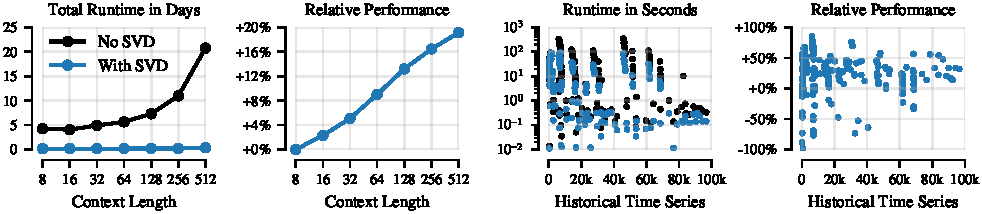
\includegraphics[width=6.75in]{fig/gift_eval.pdf}
    \caption{Runtime and performance statistics of Empirical GP on the GIFT-Eval time series forecasting benchmark.
    \textbf{Left:} As the context length increases, SVD acceleration significantly decreases runtime to a virtually negligible amount.
    \textbf{Left middle:} Increasing the context length consistently improves the performance of Empirical GP relative to itself with a shorter context length.
    \textbf{Right middle:} SVD acceleration delivers consistent runtime improvements for varying amounts of historical data.
    \textbf{Right:} Increasing the amount of historical data tends to improve and stabilize the performance of Empirical GP relative to the Seasonal Naive baseline.}
    \label{fig:gift_eval}
\end{figure*}

\begin{table*}[ht]
\caption{Average ranks (mean $\pm$ standard error) of various models on the GIFT-Eval time series forecasting benchmark, by domain and overall. Empirical GP (ours) achieves the highest rank among statistical models, 
and 
outperforms four out of eight deep learning baselines
% {\bf outperforms 4 out of 8 deep learning baselines}.
}
\label{tab:gift_eval}
\small
\centering
\setlength{\tabcolsep}{4pt}
\begin{adjustbox}{max width=\textwidth}
\begin{tabular}{ l l | c c c c c c c | c c c | c}
\toprule
& Model & Econ/Fin & Energy & Healthcare & Nature & Sales & Transport & Web/CloudOps & Overall \\
\midrule
\multirow{8}{*}{\rotatebox[origin=c]{90}{Statistical Models}} & Naive & 10.17 $\pm$ 0.80 & 12.75 $\pm$ 0.54 & 12.40 $\pm$ 1.19 & 14.53 $\pm$ 0.38 & 14.75 $\pm$ 0.22 & 15.27 $\pm$ 0.18 & 11.65 $\pm$ 0.57 & 13.09 $\pm$ 0.28 \\
 & Gaussian RBF GP & 14.83 $\pm$ 0.15 & 11.97 $\pm$ 0.68 & 13.80 $\pm$ 0.33 & 10.73 $\pm$ 0.57 & 10.75 $\pm$ 0.65 & 12.20 $\pm$ 0.40 & 13.55 $\pm$ 0.60 & 12.36 $\pm$ 0.30 \\
 & Auto ETS & 5.67 $\pm$ 1.37 & 10.59 $\pm$ 0.86 & 4.80 $\pm$ 1.53 & 11.93 $\pm$ 1.13 & 12.50 $\pm$ 1.15 & 13.07 $\pm$ 0.57 & 11.75 $\pm$ 0.76 & 10.90 $\pm$ 0.46 \\
 & Spectral Mixture GP & 13.17 $\pm$ 0.60 & 10.53 $\pm$ 0.63 & 14.00 $\pm$ 0.63 & 9.20 $\pm$ 0.76 & 9.50 $\pm$ 1.35 & 9.20 $\pm$ 0.65 & 12.70 $\pm$ 0.75 & 10.87 $\pm$ 0.35 \\
 & Auto Theta & 4.50 $\pm$ 0.87 & 11.75 $\pm$ 0.72 & 8.00 $\pm$ 1.33 & 11.73 $\pm$ 0.75 & 9.00 $\pm$ 1.27 & 13.47 $\pm$ 0.50 & \underline{8.15 $\pm$ 1.11} & 10.52 $\pm$ 0.45 \\
 & Seasonal Naive & 7.50 $\pm$ 1.17 & 7.88 $\pm$ 0.43 & 9.40 $\pm$ 1.34 & 11.93 $\pm$ 0.37 & 13.25 $\pm$ 0.41 & 11.27 $\pm$ 0.43 & 9.70 $\pm$ 0.90 & 9.68 $\pm$ 0.32 \\
 & Auto Arima & \underline{3.50 $\pm$ 0.84} & \underline{7.53 $\pm$ 0.49} & \underline{4.60 $\pm$ 1.40} & 9.67 $\pm$ 0.91 & \underline{8.25 $\pm$ 1.14} & 10.93 $\pm$ 0.46 & 10.45 $\pm$ 0.81 & 8.62 $\pm$ 0.37 \\ 
 & Empirical GP (ours) & 8.67 $\pm$ 1.26 & 7.72 $\pm$ 0.85 & 5.20 $\pm$ 1.68 & \underline{7.73 $\pm$ 0.60} & 8.50 $\pm$ 1.44 & \underline{5.87 $\pm$ 0.32} & 8.50 $\pm$ 1.18 & \textbf{7.56 $\pm$ 0.42} \\
\midrule
\multirow{8}{*}{\rotatebox[origin=c]{90}{Deep Learning}} & Crossformer & 16.00 $\pm$ 0.00 & 9.62 $\pm$ 0.87 & 11.60 $\pm$ 2.66 & 7.60 $\pm$ 1.54 & 15.75 $\pm$ 0.22 & 8.00 $\pm$ 1.85 & 7.75 $\pm$ 0.64 & 9.42 $\pm$ 0.56 \\
 & DLinear & 11.67 $\pm$ 0.45 & 9.03 $\pm$ 0.37 & 10.00 $\pm$ 1.26 & 8.80 $\pm$ 0.67 & 8.75 $\pm$ 0.74 & 9.53 $\pm$ 0.46 & 8.80 $\pm$ 0.63 & 9.23 $\pm$ 0.24 \\
 & N-BEATS & 7.83 $\pm$ 1.12 & 9.19 $\pm$ 0.50 & 9.20 $\pm$ 0.95 & 8.73 $\pm$ 0.69 & 6.50 $\pm$ 1.30 & 7.67 $\pm$ 0.36 & 6.90 $\pm$ 0.52 & 8.22 $\pm$ 0.27 \\
 & DeepAR & 9.83 $\pm$ 1.52 & 9.56 $\pm$ 0.82 & 6.80 $\pm$ 1.86 & 6.93 $\pm$ 1.27 & 3.00 $\pm$ 0.35 & 4.40 $\pm$ 0.83 & 8.10 $\pm$ 1.05 & 7.66 $\pm$ 0.49 \\
 & TiDE & 11.33 $\pm$ 0.84 & 6.16 $\pm$ 0.66 & 9.60 $\pm$ 1.82 & 7.80 $\pm$ 1.03 & 8.25 $\pm$ 1.43 & 5.80 $\pm$ 0.51 & 7.00 $\pm$ 0.60 & 7.11 $\pm$ 0.36 \\
 & TFT & 3.83 $\pm$ 0.72 & 4.22 $\pm$ 0.46 & 5.60 $\pm$ 1.66 & 3.00 $\pm$ 0.42 & 3.25 $\pm$ 0.74 & \underline{2.53 $\pm$ 0.26} & 4.65 $\pm$ 0.78 & 3.87 $\pm$ 0.27 \\
 & iTransformer & 4.17 $\pm$ 0.96 & 4.34 $\pm$ 0.73 & 6.20 $\pm$ 1.82 & 2.93 $\pm$ 0.68 & 2.25 $\pm$ 0.54 & 3.40 $\pm$ 0.35 & 3.35 $\pm$ 0.65 & 3.77 $\pm$ 0.33 \\
 & PatchTST & \underline{3.33 $\pm$ 0.61} & \underline{3.16 $\pm$ 0.46} & \underline{4.80 $\pm$ 1.11} & \underline{2.73 $\pm$ 0.32} & \underline{1.75 $\pm$ 0.41} & 3.40 $\pm$ 0.32 & \underline{3.00 $\pm$ 0.43} & \textbf{3.13 $\pm$ 0.21} \\
\bottomrule
\end{tabular}
\end{adjustbox}
\vspace{-1.5ex}
\end{table*}


For a quantitative evaluation, we consider the GIFT-Eval time series forecasting benchmark~\citep{aksu2024gifteval}, which consists of 97 datasets, spanning seven domains, ten frequencies, and a total of 144,000 time series with 177 million data points.
The seven domains are Econ/Fin, Energy, Healthcare, Nature, Sales, Transport, and Web/CloudOps, and each dataset has a fixed prediction length which is associated with short, medium, or long-term forecasts.
We do not consider the additionally provided pre-training dataset.

We consider the same baseline methods as \citet{aksu2024gifteval}, incorporating the statistical models Naive, Seasonal Naive \citep{hyndman2018forecasting}, Auto Arima, Auto ETS, and Auto Theta \citep{garza2022statsforecast}.
We also include a GP with Gaussian RBF kernel and a GP using the spectral mixture kernel with four components \citep{wilson2013gaussian}.
Furthermore, following \citet{aksu2024gifteval}, we also include eight deep learning baselines, namely DeepAR \citep{salinas2020deepar}, TFT \citep{lime2021tft}, TiDE \citep{das2023tide}, N-BEATS \citep{oreshkin2020nbeats}, PatchTST \citep{nie2023patchtst}, DLinear \citep{zeng2023transformers}, Crossformer \citep{zhang2023crossformer}, and iTransformer \citep{liu2024itransformer}.

Due to the heterogeneity of datasets in the GIFT-Eval benchmark, we extract subseries to be used as historical data using a sliding window approach akin to \Cref{sec:handcrafted_kernels}.
In particular, we set the window size to be the sum of context length and prediction length, where the former is a hyperparameter and the latter is specific to each dataset.
Furthermore, we extract independent sets of subseries for each dataset and set the maximum number of subseries per dataset to 100,000.
Subseries are selected uniformly at random without replacement, with frequencies proportional to the lengths of individual time series.
In other words, we extract more subseries from longer time series in the training data and fewer from shorter ones.
For multivariate time series, we extract independent sets of subseries corresponding to each output.
To obtain a fair comparison to GP baselines, we optimize kernel hyperparameters, such as lengthscales, amplitudes, and spectral mixture weights, on the same set of subseries which is used as historical data for Empirical GP.

Following \citet{aksu2024gifteval}, we evaluate models by ranking them based on their continuous ranked probability score (CRPS) relative to the Seasonal Naive baseline.
\Cref{tab:gift_eval} reports the mean and standard error of average ranks across models, per domain and overall.
Notably, the Empirical GP achieves the highest overall average rank across the category of statistical models, and surprisingly outperforms four out of the eight deep learning models.
Crucially, the ranks reported in \Cref{tab:gift_eval} are computed jointly across all models simultaneously, adhering to the standard GIFT-Eval evaluation protocol~\citep{aksu2024gifteval}. This allows a direct comparison between the statistical and deep learning blocks.

% The competitiveness of Empirical GPs becomes even more prominent when evaluating resource requirements. While deep learning models like PatchTST and iTransformer feature millions of trainable parameters and require substantial training budgets on multi-GPU nodes (frequently exceeding dozens of hours on clusters of NVIDIA A100 GPUs for a complete benchmark run), our dense interpolation variant requires \emph{zero gradient-based optimization parameters}. It derives its full predictive power directly from closed-form sample statistics, executing entirely on standard CPUs in less than 10 hours across all 97 datasets combined.

We attribute this competitiveness to the Empirical GP's explicit modeling of the autocorrelation patterns that dominate time series data. Conversely, deep learning (DL) baselines trained from scratch must implicitly learn these dependencies, often resulting in sample inefficiency and optimization instability. While massive pre-trained foundation models define the state-of-the-art, our results highlight that the Empirical GP remains surprisingly competitive to canonical DL baselines, {\it trained on the same data},
despite requiring no gradient-based optimization—offering a robust and exceedingly simple complement to complex neural architectures.

\Cref{fig:gift_eval} illustrates the effects of varying the context length and the number of historical subseries.
Without SVD acceleration from \Cref{subsec:egps:em}, the runtime of the Empirical GP increases significantly as the context length increases.
Using SVD acceleration results in virtually negligible runtime.
Additionally, increasing the context length improves the performance of the Empirical GP.
However, given a fixed amount of training data, increasing the context length implies fewer historical subseries, resulting in a trade-off.
In terms of the number of historical subseries, \Cref{fig:gift_eval} shows that SVD acceleration leads to consistent runtime improvements across various numbers of subseries, and that performance tends to improve and become more stable as the amount of historical data increases.

\subsection{Learning Curve Extrapolation on LCBench}
\label{sec:lcbench_experiments}
To demonstrate that Empirical GPs can also leverage sparsely observed historical data,
%via methods from \Cref{subsec:egps:em},
we next consider the task of learning curve extrapolation.
This may naturally feature sparsely observed historical data, e.g., due to infrequent logging or early stopping of jobs.
We simulate this setting using data from LCBench~\citep{zimmer2021auto}, which provides learning curve data for neural networks trained for 50 epochs across 35 different datasets with 2,000 randomly sampled hyperparameter configurations per dataset.

For each dataset, we extrapolate partially observed learning curves on a test split with 1,000 examples.
From the remaining curves, we construct historical data for the Empirical GP.
To simulate sparse historical data due to early stopping, we provide 60\% of historical curves as fully observed and truncate the remaining 40\% uniformly at random between 20\% to 80\% of the total number of epochs.

We compare Empirical GPs against extrapolation via power laws and LC-PFNs~\citep{adriaensen2023efficient}, a foundation model specifically pre-trained for learning curve extrapolation. In addition, we include the naive baseline of predicting the last observed value, which converges to the ground truth as the observed fraction approaches 100\%.

\Cref{fig:lcbench_relative} shows results on the validation set in terms of RMSE and CRPS. The Empirical GP clearly outperforms all baselines both in terms of mean prediction and uncertainty calibration, especially in the regime when only a small fraction of the learning curve has been observed.

\begin{figure}[ht]
    \centering
    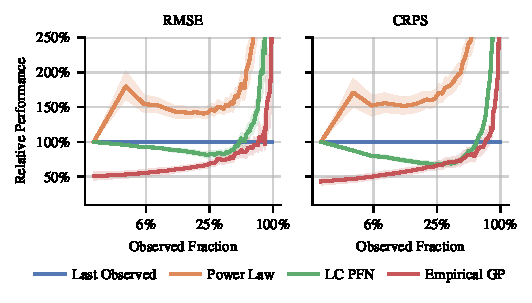
\includegraphics[width=\columnwidth]{fig/lcbench/Train_val_accuracy/relative_score.pdf}
    \caption{Performance metrics, RMSE (left) and CRPS (right), relative to the ``last observed'' baseline (lower is better), aggregated across all datasets, on the learning curve extrapolation problem.}
    \label{fig:lcbench_relative}
\end{figure}

\Cref{fig:lcbench_rank} ablates the performance of the Empirical GP as a function of both the number of historical learning curves available and their completeness (proportion that are fully observed). As expected, greater completeness leads to better prediction quality. Further, we observe approximate log-linear improvement in average percentile rank as a function of the number of historical curves.

\begin{figure}[ht!]
    \centering
    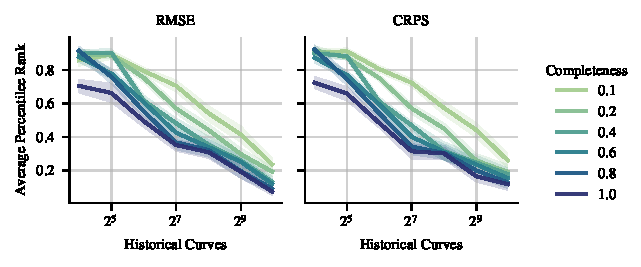
\includegraphics[width=\columnwidth]{fig/lcbench/Train_val_accuracy/ablations_avg_rank.pdf}
    \caption{Percentile ranks of performance metrics RMSE (left) and CRPS (right) at 40\% observed, aggregated across all datasets, on the LCBench learning curve extrapolation problem.}
    \label{fig:lcbench_rank}
    \vspace{-2ex}
\end{figure}

\paragraph{Comparison to GP Meta-Learning Baselines}
% \label{sec:meta_learning_baselines}

To further evaluate the effectiveness of Empirical GPs against frameworks explicitly designed to optimize across task corpuses, we benchmark our method against HyperBO~\citep{wang2024hyperbo} and PACOH~\citep{rothfuss2021pacoh} (using both its MAP and SVGD variants) on the 1D learning curve extrapolation task. The detailed tabular statistics tracking predictive accuracy (RMSE), uncertainty calibration (CRPS), exact dataset win counts, and runtime profiles across multiple observation splits are provided in Appendix~\ref{apd:additional_experiments}.

Our non-parametric estimator demonstrates substantial benefits over parametric architectures across these tasks. Specifically, Empirical GP scores the highest total dataset win count across the benchmark, achieving top-tier accuracy on 60 datasets compared to 39 for HyperBO and 18 for PACOH-SVGD. Furthermore, our model maintains the lowest overall mean CRPS error profile, confirming that the data-driven empirical prior produces well-calibrated posterior distributions. Mechanically, because our EM loop relies on stable, closed-form updates, it completely avoids the complex, non-convex optimization landscapes of deep neural kernels. This translates to exceptional speedups, allowing our model to achieve full convergence over 100$\times$ faster than particle-based methods like PACOH-SVGD.

\subsection{7D Machine Learning Hyperparameter Modeling}
\label{sec:higher_dim_experiments}

To evaluate how Empirical GPs scale to higher-dimensional input spaces where uniform grid discretization is no longer tractable, we evaluate our continuous-domain EM-EGP variant with a fitted additive base kernel (\Cref{apd:base_augmented}) on a 7-dimensional hyperparameter optimization task from LCBench~\citep{zimmer2021auto}. Here, the model maps 7 continuous black-box hyperparameter dimensions of a neural network directly to its final validation accuracy.

Instead of configuring a rigid coordinate grid, the reference anchor points $\mathbf{Z}$ are chosen as a random subset ($M = 100$) of historically observed input configurations across 30 meta-training datasets. We evaluate downstream extrapolation performance on 5 held-out evaluation datasets across varying local training sample sizes $n_{\text{train}} \in \{5, 10, 20, 50, 100\}$, using $n_{\text{test}} = 50$ configurations for validation evaluation.

\begin{table}[ht]
\small
\centering
\caption{Negative Log-Likelihood (NLL) on 7D LCBench.}
\label{tab:hd_nll}
\setlength{\tabcolsep}{4pt}
\begin{tabular}{lcccc}
\toprule
$n_{\text{train}}$ & Empirical GP & HyperBO & Pretrained GP & Vanilla GP \\
\midrule
5   & \textbf{-0.039} & 0.628 & 0.458  & 0.651 \\
10  & \textbf{-0.150} & 0.547 & 0.155  & 0.447 \\
20  & \textbf{-0.232} & 0.497 & 0.166  & 2.137 \\
50  & \textbf{-0.361} & 0.442 & -0.084 & 0.469 \\
100 & \textbf{-0.415} & 0.418 & -0.172 & 0.042 \\
\bottomrule
\end{tabular}
\end{table}

As compiled in Table~\ref{tab:hd_nll}, EM-EGP scales robustly to higher-dimensional parameter spaces without requiring structured input alignments. It provides significantly better-calibrated predictive distributions, yielding drastically lower Negative Log-Likelihood (NLL) values across all training sizes compared to alternative methods. This performance is achieved with highly efficient compute overhead, requiring only 9.3 seconds for meta-prior training on standard CPUs. Due to space constraints, the corresponding Root Mean Squared Error (RMSE) accuracy metrics -- where EM-EGP demonstrates strong data efficiency in the sparse-data regime ($n_{\text{train}} \le 20$)
--
are deferred to Appendix~\ref{apd:additional_experiments}.

%%%%%%%%%%%%%%%%%%%%%%%%%%%%%%%%%%%%%%%%%%%%%%%%%%%%%%%%%%%%%%%%%%%%%%%%%%%%%%
\section{Conclusion}
\label{sec:Conclusion}

% We studied Empirical Gaussian Processes, a principled framework for learning non-parametric GP priors from a collection of related datasets. Our contributions provide key advancements in terms of understanding and practical applicability of this approach.

We studied Empirical Gaussian Processes, a principled framework for learning non-parametric GP priors from related datasets. Our work advances both the theoretical understanding and practical applicability of this approach.

We provide a theoretical foundation, proving that Empirical GPs converge to the best Gaussian approximation of the true data-generating process. Our method provides closed-form updates that avoid compute-intensive neural-network based techniques such as HyperBO and Deep Kernel Learning. In the general case of non-shared inputs, the EM algorithm typically converges in a few iterations and scales linearly in the number of data sets, enabling efficient learning from large collections of historical data.
For dense observations, we achieve strong modeling performance through a simple algorithm without EM-steps. These results hold even using interpolation to deal with non-uniform observations.

Our experiments on time series forecasting and learning curve extrapolation demonstrate that Empirical GPs achieve performance that is competitive with multiple recent deep learning baselines on practically highly relevant problems while requiring orders of magnitude less training time.

% \textbf{Limitations and future work.} Our current analysis assumes the underlying process has finite second moments, which excludes heavy-tailed distributions. The extension to new inputs via Nystr\"om-style interpolation inherits the smoothness of the initial kernel, which may be overly restrictive in some settings. Future work could explore nonparametric smoothing of the empirical covariance (analogous to PACE) and adaptive selection of the regularization parameter $\nu$.

% \paragraph{Limitations and Future Work}
% Empirical GPs target a strategic spot between sparse data regimes and massive big-data environments. However, several limitations merit discussion:
% \begin{itemize}
%     \item \textbf{Data Availability:} In settings where historical realizations are scarce, the empirical covariance matrix can become ill-conditioned or singular, requiring fallback regularization schemes like the Inverse-Wishart prior.
%     \item \textbf{Dimensionality and Inducing Points:} The dense geometric interpolation approach (Section~\ref{sec:discrete_observations}) is explicitly restricted to low-dimensional contexts. For higher-dimensional domains, a uniform grid over $Z$ becomes intractable due to the curse of dimensionality. While we show in Appendix~\ref{apd:additional_experiments} that selecting a random subset of historical points offers an effective workaround, future research will explore optimization of $Z$ via K-means or variational Type-II MLE methods.
%     \item \textbf{Comparison to Structural Non-Stationary Kernels:} Expressive alternatives like Gibbs kernels parameterize non-stationarity via explicitly defined spatially-varying lengthscale functions. Empirical GPs offer an alternative paradigm by directly optimizing the full matrix structure non-parametrically from data, which provides unparalleled shape flexibility but incurs a cubic computation cost $\mathcal{O}(M^3)$ with respect to the reference set size during EM loops.
% \end{itemize}

\paragraph{Limitations and Future Work}
Empirical GPs target a middle ground between data-scarce regimes and
large-corpus regimes where foundation models are more expressive. With few
historical realizations, the empirical covariance is high-variance and can be
singular; we address this with a trace-matched shrinkage M-step that is exactly
MAP-EM under an Inverse-Wishart prior (\Cref{apd:shrinkage}).
The dense interpolation variant (\Cref{sec:discrete_observations}) needs
a reference grid and is thus limited to low dimensions.
Leveraging a random subset of historical inputs as reference
points is effective (\Cref{apd:additional_experiments}).
Learning $\mathbf{Z}$ via $k$-means or Type-II MLE is left to future work.
EM only recovers the best \emph{Gaussian} fit under
finite second moments; heavy-tailed or non-Gaussian structure, which structured
kernels (e.g., Gibbs) or non-Gaussian processes can target, is beyond our scope.

% We studied Empirical Gaussian Processes, a principled framework for learning non-parametric GP priors from related datasets. Our work advances both the theoretical understanding and practical applicability of this approach.

% Theoretically, we proved that the Empirical GP converges to the best Gaussian approximation of the true data-generating process. Practically, our method provides closed-form updates that avoid the compute-intensive neural-network techniques used by HyperBO and Deep Kernel Learning. In the general case of non-shared sample locations, our EM algorithm converges in just a few iterations and scales linearly with the number of datasets, enabling efficient learning from large historical collections. For the case of dense observations, we show that the EM algorithm is unnecessary, and that we achieve strong performance through a simpler algorithm, even when using interpolation to arrange non-uniform observations on a grid.

% Our experiments on time series forecasting and learning curve extrapolation demonstrate that Empirical GPs achieve performance competitive with recent deep learning baselines on real-world benchmarks, while requiring orders of magnitude less training time.

% Limitations and future work. Empirical GPs occupy a “sweet spot” between regimes where little historical data is available, and those with massive amounts of data. In the former, Empirical GPs may find it challenging to estimate the prior, necessitating stronger parametric assumptions. In the latter, foundation models trained on massive corpuses can achieve higher expressiveness—though they may struggle with out-of-distribution data due to the limits of in-context learning.


\clearpage

% % Acknowledgements should only appear in the accepted version.
\section*{Acknowledgements}
We thank Samuel Müller for helpful discussions and insights about the GIFT-Eval benchmark.
% \textbf{Do not} include acknowledgements in the initial version of the paper
% submitted for blind review.

% If a paper is accepted, the final camera-ready version can (and usually should)
% include acknowledgements.  Such acknowledgements should be placed at the end of
% the section, in an unnumbered section that does not count towards the paper
% page limit. Typically, this will include thanks to reviewers who gave useful
% comments, to colleagues who contributed to the ideas, and to funding agencies
% and corporate sponsors that provided financial support.

\section*{Impact Statement}
This paper presents work whose goal is to advance the field of Machine
Learning. There are many potential societal consequences of our work, none
which we feel must be specifically highlighted here.


% In the unusual situation where you want a paper to appear in the
% references without citing it in the main text, use \nocite

\bibliography{references}
\bibliographystyle{icml2026}

%%%%%%%%%%%%%%%%%%%%%%%%%%%%%%%%%%%%%%%%%%%%%%%%%%%%%%%%%%%%%%%%%%%%%%%%%%%%%%%
%%%%%%%%%%%%%%%%%%%%%%%%%%%%%%%%%%%%%%%%%%%%%%%%%%%%%%%%%%%%%%%%%%%%%%%%%%%%%%%
% APPENDIX
%%%%%%%%%%%%%%%%%%%%%%%%%%%%%%%%%%%%%%%%%%%%%%%%%%%%%%%%%%%%%%%%%%%%%%%%%%%%%%%
%%%%%%%%%%%%%%%%%%%%%%%%%%%%%%%%%%%%%%%%%%%%%%%%%%%%%%%%%%%%%%%%%%%%%%%%%%%%%%%
\newpage
\appendix
\onecolumn

%%%%%%%%%%%%%%%%%%%%%%%%%%%%%%%%%%%%%%%%%%%%%%%%%%%%%%%%%%%%%%%%%%%%%%%%%%%%%%
\section{Theory}
\label{apd:theory}

\subsection{Function-Space View}
In this section, we provide derivations for our theoretical results from \Cref{sec:egps}.

Let $(\domain, \rho)$ be a compact metric space.
Let $C(\domain)$ denote the separable Banach space of continuous real-valued functions on $\domain$, equipped with the supremum norm $\Vert h \Vert_{\infty} = \sup_{\vx \in \domain} | h(\vx) |$ for all $h \in C(\domain)$.
Let $f$ be drawn from a stochastic process indexed by $\domain$ with mean function $m(\vx) = \mathbb{E}[f(\vx)]$ and covariance function $k(\vx, \vx') = \mathrm{Cov}(f(\vx), f(\vx'))$.
We assume that $f$ has almost surely continuous sample paths on $\domain$ and finite second moments $\mathbb{E}[ \Vert f \Vert_{\infty}^2 ] < \infty$.
Note that, the latter is implied by Fernique's theorem \citep{fernique1970} if $f$ follows a \emph{Gaussian} process.
Let $f_1, ..., f_\K$ be $\K$ \iid sample paths of $f$.
We define the \emph{empirical} mean function $m_\K$ and the \emph{empirical} covariance function $k_{\K}$ as
\begin{align*}
    m_\K(\vx)
    = \frac{1}{\K} \sum_{i=1}^{\K} f_i(\vx), &&
    k_\K(\vx, \vx')
    = \frac{1}{\K} \sum_{i=1}^{\K} (f_i(\vx) - m_\K(\vx))(f_i(\vx') - m_\K(\vx')).
\end{align*}
We first show that the empirical mean and covariance functions almost surely converge uniformly to their true counterparts.
\begin{restatable}{lemma}{MeanCovarConvergence}
\label{thm:mean_covar_convergence}
Suppose that $f$ has almost surely continuous sample paths on $\domain$ and finite second moments $\mathbb{E}[ \Vert f \Vert_{\infty}^2 ] < \infty$.
Note that, the latter is implied by Fernique's theorem \citep{fernique1970} if $f$ is a \emph{Gaussian} process. In the limit of $\K \to \infty$, we have
\begin{equation*}
    \Vert m_\K - m \Vert_{\infty} \xrightarrow{\mathrm{a.s.}} 0
    \quad \text{and} \quad
    \Vert k_\K - k \Vert_{\infty} \xrightarrow{\mathrm{a.s.}} 0,
\end{equation*}
that is, the empirical mean and covariance function almost surely converge uniformly to their true counterparts.
\end{restatable}
\begin{proof}
First, note that the sample paths $f_1, ..., f_\K$ are \iid random elements taking values in the separable Banach space $C(\domain)$.
Applying Mourier's strong law of large numbers \citep{mourier1953}, we obtain
\begin{equation*}
    \left\Vert \frac{1}{\K} \sum_{i=1}^\K f_i - \mathbb{E}[f] \right\Vert_{\infty} \xrightarrow{\mathrm{a.s.}} 0
    \quad \text{in } C(\domain).
\end{equation*}
Since $\mathbb{E}[f(\vx)] = m(\vx)$, we have $\Vert m_\K - m \Vert_{\infty} \xrightarrow{\mathrm{a.s.}} 0$.

For the empirical covariance function, we consider the random element $h = f \otimes f$, defined by $h(\vx, \vx') = f(\vx)f(\vx')$, where $f \in C(\domain)$ implies $h \in C(\domain \times \domain)$.
Additionally, since $\domain$ is a compact metric space, $\domain \times \domain$ is also a compact metric space, implying that $C(\domain \times \domain)$ is a separable Banach space with supremum norm
\begin{equation*}
    \Vert h \Vert_{\infty}
    = \sup_{(\vx, \vx') \in \domain \times \domain} | h(\vx, \vx') |
    = \Vert f \Vert_{\infty}^2.
\end{equation*}
Since $\mathbb{E} [\Vert f \Vert_{\infty}^2] < \infty$, we have $\mathbb{E} [\Vert h \Vert_{\infty}] < \infty$.
By applying Mourier's strong law of large numbers \citep{mourier1953} again, we obtain
\begin{equation*}
    \left\Vert \frac{1}{\K} \sum_{i=1}^\K h_i - \mathbb{E}[h] \right\Vert_{\infty} \xrightarrow{\mathrm{a.s.}} 0
    \quad \text{in } C(\domain \times \domain),
\end{equation*}
with $\mathbb{E}[h(\vx, \vx')] = \mathbb{E}[f(\vx)f(\vx')] = k(\vx, \vx') + m(\vx) m(\vx')$.

Since the mapping $(u, v) \mapsto u \otimes v$ from $C(\domain) \times C(\domain) \to C(\domain \times \domain)$ is continuous, $\Vert m_\K - m \Vert_{\infty} \xrightarrow{\mathrm{a.s.}} 0$ implies
\begin{equation*}
    m_\K(\vx) m_\K(\vx') \xrightarrow{\mathrm{a.s.}} m(\vx) m(\vx')
    \quad \text{uniformly on } \domain \times \domain,
\end{equation*}
via the continuous mapping theorem.
Combining the two results above with the continuity of subtraction yields
\begin{equation*}
    k_\K \xrightarrow{\mathrm{a.s.}} (k + m \otimes m) - (m \otimes m) = k \quad \text{uniformly on } \domain \times \domain,
\end{equation*}
which gives the claim.
\end{proof}
For any finite set of points $\vx_1, ..., \vx_N \in \domain$, we define
\begin{align*}
    \mathbf{m} &=
    \begin{bmatrix}
        m(\vx_i)
    \end{bmatrix}_{i=1}^N, &
    \mathbf{m}_\K &=
    \begin{bmatrix}
        m_\K(\vx_i)
    \end{bmatrix}_{i=1}^N, &
    \mathbf{K} &=
    \begin{bmatrix}
        k(\vx_i, \vx_j)
    \end{bmatrix}_{i,j=1}^N, &
    \mathbf{K}_\K &=
    \begin{bmatrix}
        k_\K(\vx_i, \vx_j)
    \end{bmatrix}_{i,j=1}^N.
\end{align*}
Note that $k_\K$ is a valid covariance function, because $\mathbf{K}$ is positive semi-definite, that is, for any $\mathbf{u} \in \mathbb{R}^n$
\begin{equation*}
    \mathbf{u}^\mathsf{T} \mathbf{K}_\K \mathbf{u}
    = \frac{1}{\K} \sum_{i=1}^\K \biggl( \sum_{j=1}^N u_j ( f_i(\vx_j) - m_\K(\vx_j) ) \biggr)^2 \geq 0.
\end{equation*}
Next, we show that the finite-dimensional multivariate normal random variable $\mathbf{g}_S \sim \mathcal{N}(\mathbf{m}_S, \mathbf{K}_S)$, induced by the empirical mean and covariance functions, converges in distribution to $\mathbf{g} \sim \mathcal{N}(\mathbf{m}, \mathbf{K})$, the corresponding multivariate normal random variable induced by the true mean and covariance functions.
\begin{restatable}{lemma}{FiniteDistConvergence}
\label{thm:finite_dist_convergence}
For almost every sequence of sample paths $\{ f_i \}_{i=1}^S$ and any finite set of points $\vx_1, ..., \vx_N \in \domain$,
\begin{equation*}
    \mathbf{g}_S \xrightarrow{d} \mathbf{g} \quad \text{as} \quad S \to \infty,
\end{equation*}
that is, the multivariate normal random variable induced by the empirical mean and covariance functions converges in distribution to the corresponding multivariate normal random variable induced by the true mean and covariance function.
\end{restatable}
\begin{proof}
The characteristic function of $\mathbf{g}_S \sim \mathcal{N}(\mathbf{m}_S, \mathbf{K}_S)$ is given by
\begin{equation*}
    \varphi_\K(\mathbf{t}) = \exp \left( i \mathbf{t}^{\mathsf{T}} \mathbf{m}_\K - \frac{1}{2} \mathbf{t}^{\mathsf{T}} \mathbf{K}_\K \mathbf{t}  \right), \quad \forall \mathbf{t} \in \mathbb{R}^N.
\end{equation*}
Applying \Cref{thm:mean_covar_convergence}, we obtain element-wise convergence of $\mathbf{m}_S \to \mathbf{m}$ and $\mathbf{K}_\K \to \mathbf{K}$ for almost every realization of the sample paths.
By continuity of $\varphi_\K$, we obtain pointwise convergence of
\begin{equation*}
    \varphi_\K(\mathbf{t}) \to \varphi(\mathbf{t})
    = \exp \left( i \mathbf{t}^{\mathsf{T}} \mathbf{m} - \frac{1}{2} \mathbf{t}^{\mathsf{T}} \mathbf{K} \mathbf{t}  \right), \quad \forall \mathbf{t} \in \mathbb{R}^N,
\end{equation*}
for almost every realization of $\{f_i\}_{i=1}^S$, as $\K \to \infty$.
Observing that $\varphi$ is the characteristic function of $\mathbf{g} \sim \mathcal{N}(\mathbf{m}, \mathbf{K})$ and continuous at $\mathbf{t} = \mathbf{0}$, we apply Lévy's continuity theorem \citep{levy1925} and conclude the claim.
\end{proof}
Let $\mathcal{GP}\bigl(m_\K, k_\K\bigr)$ be a GP defined by the empirical mean function $m_\K$ and empirical covariance function $k_\K$, conditioned on observed sample paths $f_1, ..., f_\K$.
We refer to $\mathcal{GP}\bigl(m_\K, k_\K\bigr)$ as Empirical GP.
Additionally, let $\mathcal{GP}\bigl(m, k)$ be a Gaussian process defined by the true mean function $m$ and true covariance function $k$.
We refer to $\mathcal{GP}\bigl(m, k)$ as \emph{limiting} GP.
\WeakConvergence*
\begin{proof}
To establish the weak convergence of $\mathcal{GP}\bigl(m_\K, k_\K\bigr) \rightharpoonup \mathcal{GP}\bigl(m, k)$ in $C(\domain)$, we must verify the convergence of finite-dimensional distributions and the tightness of the sequence of measures induced by $\{ \mathcal{GP}\bigl(m_\K, k_\K\bigr) \}_{\K=1}^\infty$.
The convergence of finite-dimensional distributions is established directly by \Cref{thm:finite_dist_convergence}.
For tightness in $C(\mathcal X)$, Dudley’s condition implies $\mathcal{GP}\bigl(m, k)$ is supported on $C(\mathcal X)$.
Uniform convergence $k_\K\to k$, established by \Cref{thm:mean_covar_convergence}, implies $d_{k_\K}\to d_k$ uniformly, and thus the entropy integrals of $(\mathcal X,d_{k_\K})$
are uniformly bounded for all sufficiently large $\K$.
By Dudley’s theorem \citep{dudley1967}, $\{ \mathcal{GP}\bigl(m_\K, k_\K\bigr) \}_{S=1}^\infty$ is tight in $C(\mathcal X)$.
Finally, convergence of finite-dimensional distributions plus tightness yields weak convergence in $C(\mathcal X)$ via Prokhorov's theorem \citep{prokhorov1956}.
\end{proof}
This weak convergence implies weak convergence of posteriors under Bayesian inference.
\begin{restatable}{corollary}{PosteriorConvergence}
\label{thm:posterior_convergence}
Given a dataset $\mathcal{D}$, for almost every sequence of sample paths $\{ \stochprocess_i \}_{i=1}^\K$, $\mathcal{GP}\bigl(m_\K, k_\K\bigr) \!\mid\! \mathcal{D} \rightharpoonup \mathcal{GP}\bigl(m, k\bigr) \!\mid\! \mathcal{D}$ as $\K \to \infty$,
that is, the posterior of $\mathcal{GP}\bigl(m_\K, k_\K\bigr)$ conditioned on $\mathcal{D}$ converges weakly to the posterior of $\mathcal{GP}\bigl(m, k\bigr)$ in $C(X)$.
\end{restatable}
\begin{proof}
The posterior mean and covariance functions are continuous mappings of the corresponding prior mean and covariance functions.
Therefore, they preserve the uniform convergence properties established by \Cref{thm:mean_covar_convergence}.
An argument analogous to \Cref{thm:weak_convergence} gives the claim.
\end{proof}
Finally, we show that the limiting Gaussian process $g$ is the best possible Gaussian approximation, in terms of KL divergence, of the true underlying stochastic process $f$.

\KLD*
\begin{proof}
Following \citep{sun2019functional}, we define the KL divergence between stochastic processes via finite-dimensional marginals,
\begin{equation*}
    D_{\mathrm{KL}} ( \mathbb{P} \;\Vert\; \mathbb{G} )
    = \sup_{\bX \subset \domain, \; |\bX| < \infty} D_{\mathrm{KL}} ( \mathbb{P}_{\samplevec_{\bX}} \;\Vert\; \mathbb{G}_{\mathbf{h}_{\bX}} ).
\end{equation*}
For any finite $\bX \subset \domain$, let $p_{\bX}$ denote the distribution of $\samplevec_{\bX}$ with mean $\boldsymbol{\mu}_{\bX}$ and covariance $\boldsymbol{\Sigma}_{\bX}$.
For a GP $\mathbb{G}$ with mean $\tilde{m}$ and covariance $\tilde{k}$, we have $\mathbf{h}_{\bX} \sim \mathcal{N}(\tilde{\boldsymbol{\mu}}_{\bX}, \tilde{\boldsymbol{\Sigma}}_{\bX})$.
Decomposing the KL divergence into entropy and cross-entropy, we have
\begin{equation*}
    D_{\mathrm{KL}} ( p_{\bX} \;\Vert\; \mathcal{N}(\tilde{\boldsymbol{\mu}}_{\bX}, \tilde{\boldsymbol{\Sigma}}_{\bX}) )
    = -H(p_{\bX}) + H(p_{\bX}, \mathcal{N}(\tilde{\boldsymbol{\mu}}_{\bX}, \tilde{\boldsymbol{\Sigma}}_{\bX})).
\end{equation*}
Since the entropy $H(p_{\bX})$ is independent of $\mathbb{G}$, minimizing the KL divergence is equivalent to minimizing the cross-entropy.
For a Gaussian target, the cross-entropy depends on $p_{\bX}$ only through its first two moments,
\begin{equation*}
    H(p_{\bX}, \mathcal{N}(\tilde{\boldsymbol{\mu}}_{\bX}, \tilde{\boldsymbol{\Sigma}}_{\bX}))
    = \frac{1}{2} \log | 2 \pi \tilde{\boldsymbol{\Sigma}}_{\bX} | + \frac{1}{2} \mathrm{tr}(\tilde{\boldsymbol{\Sigma}}_{\bX}^{-1} \boldsymbol{\Sigma}_{\bX}) + \frac{1}{2}(\boldsymbol{\mu}_{\bX} - \tilde{\boldsymbol{\mu}}_{\bX})^\top \tilde{\boldsymbol{\Sigma}}_{\bX}^{-1} (\boldsymbol{\mu}_{\bX} - \tilde{\boldsymbol{\mu}}_{\bX}).
\end{equation*}
The cross-entropy is strictly convex in the natural parameters of the Gaussian, and is uniquely minimized when $\tilde{\boldsymbol{\mu}}_{\bX} = \boldsymbol{\mu}_{\bX}$ and $\tilde{\boldsymbol{\Sigma}}_{\bX} = \boldsymbol{\Sigma}_{\bX}$.

By \Cref{thm:weak_convergence}, the mean and covariance of $\lim_{S \to \infty} \mathcal{GP}\bigl(m_\K, k_\K\bigr)$ converge to their true counterparts, such that, for every finite $\bX$, the marginal $\mathbf{g}_{\bX} \sim \mathcal{N}(\boldsymbol{\mu}_{\bX}, \boldsymbol{\Sigma}_{\bX})$ uniquely minimizes the marginal KL divergence.
Any other GP differs on some finite $\bX^*$, yielding a strictly larger KL divergence on that marginal, and hence a strictly larger supremum.
\end{proof}
\subsection{EM-based Model}
\begin{restatable}{lemma}{ShiftInterpolationPSD}[Shift-Interpolant]
\label{lem:shift_interapolant_psd}
Let the interpolated covariance at new input locations $\mathbf{X}_*$ be defined as:
\begin{equation}
    \boldsymbol{\Sigma}(\mathbf{X}_*, \mathbf{X}_*) = k(\mathbf{X}_*, \mathbf{X}_*) + \mathbf{W} \boldsymbol{\delta}_{\Sigma} \mathbf{W}^\top,
\end{equation}
where $\mathbf{W} = \mathbf{K}_{*X} \mathbf{K}_{XX}^{-1}$ and $\boldsymbol{\delta}_{\Sigma} = \boldsymbol{\Sigma} - \mathbf{K}_{XX}$.
If the EM-optimized covariance $\boldsymbol{\Sigma}$ is positive semi-definite (PSD),
and the base kernel $k(\cdot, \cdot)$ is a valid covariance function
that is positive (semi-)definite,
then $\boldsymbol{\Sigma}(\mathbf{X}_*, \mathbf{X}_*)$ is positive (semi-)definite.
\end{restatable}

\begin{proof}
We begin by expanding the definition of the interpolated covariance. Let $\mathbf{K}_{**} = k(\mathbf{X}_*, \mathbf{X}_*)$, $\mathbf{K}_{*X} = k(\mathbf{X}_*, \mathbf{X})$, and $\mathbf{K}_{XX} = k(\mathbf{X}, \mathbf{X})$. Substituting the definition of the residual $\boldsymbol{\delta}_{\Sigma}$ into the interpolation formula:
\begin{equation}
    \nonumber
\begin{aligned}
    \boldsymbol{\Sigma}(\mathbf{X}_*, \mathbf{X}_*) &= \mathbf{K}_{**} + \mathbf{W} (\boldsymbol{\Sigma} - \mathbf{K}_{XX}) \mathbf{W}^\top \\
    &= \mathbf{K}_{**} + \mathbf{W} \boldsymbol{\Sigma} \mathbf{W}^\top - \mathbf{W} \mathbf{K}_{XX} \mathbf{W}^\top.
\end{aligned}
\end{equation}

We simplify the term $\mathbf{W} \mathbf{K}_{XX} \mathbf{W}^\top$ using the definition of the weight matrix $\mathbf{W} = \mathbf{K}_{*X} \mathbf{K}_{XX}^{-1}$:
\begin{equation}
    \nonumber
    \begin{aligned}
        \mathbf{W} \mathbf{K}_{XX} \mathbf{W}^\top &= (\mathbf{K}_{*X} \mathbf{K}_{XX}^{-1}) \mathbf{K}_{XX} (\mathbf{K}_{*X} \mathbf{K}_{XX}^{-1})^\top \\
        &= \mathbf{K}_{*X} (\mathbf{K}_{XX}^{-1} \mathbf{K}_{XX}) \mathbf{K}_{XX}^{-1} \mathbf{K}_{X*} \\
        &= \mathbf{K}_{*X} \mathbf{K}_{XX}^{-1} \mathbf{K}_{X*}.
    \end{aligned}
\end{equation}
Substituting this back into the expansion above, we can rearrange the interpolated covariance as the sum of two distinct matrices, denoted $\mathbf{A}$ and $\mathbf{B}$:
\begin{equation}
    \nonumber
    \boldsymbol{\Sigma}(\mathbf{X}_*, \mathbf{X}_*) = \underbrace{\left( \mathbf{K}_{**} - \mathbf{K}_{*X} \mathbf{K}_{XX}^{-1} \mathbf{K}_{X*} \right)}_{\mathbf{A}} + \underbrace{\left( \mathbf{W} \boldsymbol{\Sigma} \mathbf{W}^\top \right)}_{\mathbf{B}}.
\end{equation}
To prove that $\boldsymbol{\Sigma}(\mathbf{X}_*, \mathbf{X}_*) \succeq 0$, it suffices to show that both $\mathbf{A}$ and $\mathbf{B}$ are positive semi-definite.

\paragraph{1. Analysis of $\mathbf{A}$ (Schur Complement)}
The matrix $\mathbf{A}$ is recognized as the conditional covariance of the base Gaussian Process at locations $\mathbf{X}_*$ given observations at $\mathbf{X}$. Consider the joint kernel matrix of the union of grid points and new points, which is PSD by the definition of the kernel function $k(\cdot, \cdot)$:
\begin{equation}
    \nonumber
    \mathbf{K}_{\text{joint}} = \begin{bmatrix} \mathbf{K}_{XX} & \mathbf{K}_{X*} \\ \mathbf{K}_{*X} & \mathbf{K}_{**} \end{bmatrix} \succeq 0.
\end{equation}
By the properties of the Schur complement, if a block matrix is PSD, the Schur complement of its principal submatrix $\mathbf{K}_{XX}$ is also PSD. Therefore:
\begin{equation}
    \nonumber
    \mathbf{A} = \mathbf{K}_{**} - \mathbf{K}_{*X} \mathbf{K}_{XX}^{-1} \mathbf{K}_{X*} \succeq 0.
\end{equation}

\paragraph{2. Analysis of $\mathbf{B}$ (Projected Learned Covariance)}
The matrix $\mathbf{B} = \mathbf{W} \boldsymbol{\Sigma} \mathbf{W}^\top$ is a congruence transformation of $\boldsymbol{\Sigma}$.
From the M-step of the EM algorithm, $\boldsymbol{\Sigma}$ is updated as a sum of posterior covariances and outer products of mean adjustments:
\begin{equation}
    \nonumber
    \boldsymbol{\Sigma}^{(t+1)} = \frac{1}{K-1} \sum_{i=1}^{K} \mathbf{C}_i + \mathbf{\tilde m}_i \mathbf{\tilde m}_i^{\top}.
\end{equation}
Since covariance matrices $\mathbf{C}_i$ and outer products $\mathbf{\tilde m}_i \mathbf{\tilde m}_i^{\top}$ are always positive semi-definite, their sum $\boldsymbol{\Sigma}$ is PSD ($\boldsymbol{\Sigma} \succeq 0$).
For any vector $\mathbf{v}$, let $\mathbf{u} = \mathbf{W}^\top \mathbf{v}$. Then:
\begin{equation}
    \nonumber
    \mathbf{v}^\top \mathbf{B} \mathbf{v} = \mathbf{v}^\top \mathbf{W} \boldsymbol{\Sigma} \mathbf{W}^\top \mathbf{v} = \mathbf{u}^\top \boldsymbol{\Sigma} \mathbf{u} \geq 0.
\end{equation}
Thus, $\mathbf{B} \succeq 0$.

\paragraph{Conclusion}
Since $\boldsymbol{\Sigma}(\mathbf{X}_*, \mathbf{X}_*) = \mathbf{A} + \mathbf{B}$ is the sum of two positive semi-definite matrices, it is itself positive semi-definite.
Further, if the base kernel $k$ is positive definite (strict inequality),
then $\boldsymbol{\Sigma}(\mathbf{X}_*, \mathbf{X}_*) \succeq \mathbf{A} \succ 0$.
\end{proof}


\subsection{Computational Complexity of the EM-Algorithm With Residual Interpolation}

Substituting the dense $\mathbf{Q}_i$ for $\sigma^2\mathbf{I}$ in
$\boldsymbol{\Sigma}_{\mathbf{X}_i,\mathbf{X}_i}$ forfeits the
low-rank-plus-diagonal structure exploited by the Woodbury identity, raising the
E-step inversion from $\mathcal{O}(M^3 + N_iM^2)$ to $\mathcal{O}(N_i^3)$ in the
large-observation regime $N_i > M$.
However, it is required to make the variance-starvation fix
consistent during training on sparse, irregular data.

\section{Additional Details of the Experiments}

\subsection{Datasets}
GIFT-Eval and LCBench are available under the Apache License 2.0. S\&P 500 data on Kaggle was retrieved under the CC0 License. The Mauna Loa dataset is available under the CC0 License.

\subsection{Baseline Implementations}
LC-PFN is available on GitHub under the MIT License at \url{https://github.com/automl/lcpfn}

\paragraph{Limitations of the baseline comparisons.}
Two properties of this protocol bound how finely the reported differences should be
read, and we state them explicitly rather than leave them implicit.

\emph{Sensitivity to pre-training budget.} Deep-kernel meta-learners are strongly
budget-dependent, and the dependence is not visible in converged metrics.
We found that increasing HyperBO's pre-training from $2\,000$ to $25\,000$ steps improved its
regret-AUC by $33\%$, with the knee near $5\,000$ steps --- while the
\emph{final} regret was flat across the whole range, so a budget chosen on a
converged metric can silently under-train the baseline. Baselines here were not
separately tuned to convergence, so their numbers should be read as a lower bound
on achievable performance rather than as a tuned ceiling.

\emph{Single pre-training run.} Where a single pre-trained prior is reused across
evaluation tasks, per-task variability does not capture uncertainty in the prior
itself: the effective sample size for comparing two \emph{priors} is one. Measuring
this directly on LCBench across five independent pre-training seeds, we observed a
prior-draw standard deviation in regret-AUC of $0.037$ for HyperBO and $0.248$ for
PACOH --- for PACOH, larger than several of the between-method gaps of interest.
Differences of this magnitude between meta-learning baselines should therefore not
be over-interpreted without multiple pre-training seeds.

Neither caveat affects the Empirical GP results, whose EM pre-training is
deterministic given the historical data and involves no such budget: we measured a
prior-draw standard deviation of exactly zero.

\subsection{Compute Usage}
One benefit of Empirical GPs is that they are quite compute-efficient. All of our  experiments were performed on Intel Cooper Lake CPUs, using less than 3,000 CPU hours in total.

\subsection{EM-Algorithm Convergence Speed}
\label{sec:em_convergence_speed}

Figure~\ref{fig:em_iteration_convergence} shows the $L_2$ norm of the difference of subsequent iterates of the EM-estimated prior mean $\mu^{(t)}$ and covariance $\Sigma^{(t)}$, as a function of the number of noisy independent incomplete datasets (\K), and for different numbers of observed data points per dataset (n).
Notably, convergence speed to a fixed-point of the EM-iterations depends on the number of observed entries $n$, compared to the size of the full latent vector $N = 128$ in this case.
Note that the reason $n = 128$ is not converging within one iteration in this case
is because this is studying the noisy case, where $\sigma^2 = 10^{-4}$,
showing that even in the full observed case,
the EM-iterations with $\sigma^2 > 0$ require a number of iterations to converge,
in order to de-noise the latent vectors $\{\samplevec_i\}$.

\begin{figure*}[ht]
    \centering
    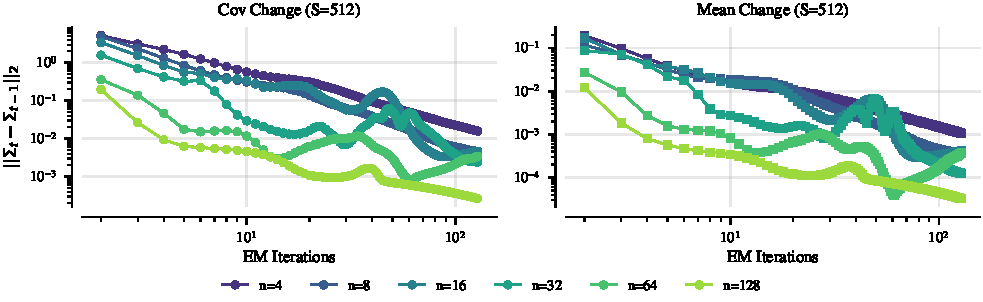
\includegraphics[width=6.75in]{fig/em_iteration_convergence.pdf}
    \caption{
        $L_2$ norm of the difference of subsequent iterates of the EM-estimated prior mean $\mu^{(t)}$ and covariance $\Sigma^{(t)}$, as a function of the number of independent incomplete datasets (\K), and for different numbers of observed data points per dataset (n).
    }
\label{fig:em_iteration_convergence}
\end{figure*}


\section{Additional Empirical Evaluations}
\label{apd:additional_experiments}

This section provides comprehensive experimental results to supplement the main text, presenting both the high-dimensional scalability accuracy metrics and the detailed 1D meta-learning baseline comparisons.

\subsection{Additional Learning Curve Extrapolation Results}

Table~\ref{tab:results_avg_rank_lc_extrapolation} shows the average rank,
and
Table \ref{tab:results_perf_metrics_lc_extrapolation} shows the performance metrics at 40\% observed fraction for the learning curve extrapolation benchmark of Section~\ref{sec:lcbench_experiments}.

\begin{table}[h]
\small
\centering
\setlength{\tabcolsep}{4pt}
\caption{Average rank for the 1D LCBench learning curve extrapolation benchmark of Section~\ref{sec:lcbench_experiments}}
\label{tab:results_avg_rank_lc_extrapolation}
\begin{tabular}{c*{8}{r}}
\toprule
 & \multicolumn{4}{c}{RMSE} & \multicolumn{4}{c}{CRPS} \\
\cmidrule(lr){2-5} \cmidrule(lr){6-9}
Observed & Last Observed & Power Law & LC PFN & Empirical GP & Last Observed & Power Law & LC PFN & Empirical GP \\
 % &  &  &  &  &  &  &  &  \\
\midrule
10\% & 2.91 $\pm$ 0.37 & 3.94 $\pm$ 0.34 & 2.14 $\pm$ 0.36 & 1.00 $\pm$ 0.00 & 3.03 $\pm$ 0.30 & 3.94 $\pm$ 0.24 & 2.00 $\pm$ 0.24 & 1.03 $\pm$ 0.17 \\
20\% & 2.91 $\pm$ 0.28 & 4.00 $\pm$ 0.00 & 2.03 $\pm$ 0.38 & 1.06 $\pm$ 0.24 & 3.03 $\pm$ 0.17 & 3.97 $\pm$ 0.17 & 1.74 $\pm$ 0.44 & 1.26 $\pm$ 0.44 \\
30\% & 2.83 $\pm$ 0.45 & 3.97 $\pm$ 0.17 & 1.97 $\pm$ 0.57 & 1.23 $\pm$ 0.55 & 2.86 $\pm$ 0.36 & 4.00 $\pm$ 0.00 & 1.69 $\pm$ 0.58 & 1.46 $\pm$ 0.66 \\
40\% & 2.80 $\pm$ 0.53 & 3.94 $\pm$ 0.24 & 2.06 $\pm$ 0.64 & 1.20 $\pm$ 0.47 & 2.83 $\pm$ 0.45 & 4.00 $\pm$ 0.00 & 1.63 $\pm$ 0.60 & 1.54 $\pm$ 0.66 \\
50\% & 2.26 $\pm$ 0.66 & 3.94 $\pm$ 0.24 & 2.43 $\pm$ 0.78 & 1.37 $\pm$ 0.73 & 2.57 $\pm$ 0.61 & 4.00 $\pm$ 0.00 & 1.91 $\pm$ 0.66 & 1.51 $\pm$ 0.82 \\
60\% & 2.31 $\pm$ 0.76 & 3.91 $\pm$ 0.28 & 2.31 $\pm$ 0.80 & 1.46 $\pm$ 0.78 & 2.29 $\pm$ 0.71 & 4.00 $\pm$ 0.00 & 2.20 $\pm$ 0.76 & 1.51 $\pm$ 0.78 \\
70\% & 2.09 $\pm$ 0.95 & 3.89 $\pm$ 0.32 & 2.54 $\pm$ 0.70 & 1.49 $\pm$ 0.66 & 1.83 $\pm$ 0.66 & 4.00 $\pm$ 0.00 & 2.57 $\pm$ 0.70 & 1.60 $\pm$ 0.77 \\
80\% & 1.89 $\pm$ 0.76 & 3.97 $\pm$ 0.17 & 2.57 $\pm$ 0.70 & 1.57 $\pm$ 0.74 & 1.51 $\pm$ 0.61 & 4.00 $\pm$ 0.00 & 2.74 $\pm$ 0.56 & 1.74 $\pm$ 0.70 \\
90\% & 1.54 $\pm$ 0.61 & 4.00 $\pm$ 0.00 & 2.89 $\pm$ 0.40 & 1.57 $\pm$ 0.56 & 1.14 $\pm$ 0.36 & 4.00 $\pm$ 0.00 & 2.97 $\pm$ 0.17 & 1.89 $\pm$ 0.40 \\
\bottomrule
\end{tabular}
\end{table}


\begin{table}[h]
\small
\centering
\setlength{\tabcolsep}{4pt}
\caption{Performance metrics at 40\% observed fraction for the 1D LCBench learning curve extrapolation benchmark of Section~\ref{sec:lcbench_experiments}}
\label{tab:results_perf_metrics_lc_extrapolation}
\begin{tabular}{l*{8}{r}}
\toprule
 & \multicolumn{4}{c}{RMSE} & \multicolumn{4}{c}{CRPS} \\
\cmidrule(lr){2-5} \cmidrule(lr){6-9}
Dataset & Last Observed & Power Law & LC PFN & Empirical GP & Last Observed & Power Law & LC PFN & Empirical GP \\
% Dataset &  &  &  &  &  &  &  &  \\
\midrule
adult & 3.1908 & 4.6024 & 1.8041 & 4.6075 & 0.0108 & 0.0285 & 0.0063 & 0.0118 \\
airlines & 3.1024 & 3.0310 & 1.9329 & 0.9740 & 0.0182 & 0.0281 & 0.0135 & 0.0092 \\
albert & 1.1373 & 1.6251 & 1.2812 & 1.1045 & 0.0089 & 0.0156 & 0.0082 & 0.0070 \\
Amazon\_employee... & 4.5946 & 8.4153 & 4.4209 & 4.5202 & 0.0270 & 0.0629 & 0.0213 & 0.0279 \\
APSFailure & 3.2776 & 6.6912 & 3.0040 & 1.5685 & 0.0103 & 0.0275 & 0.0064 & 0.0057 \\
Australian & 3.9182 & 6.9080 & 3.7916 & 2.6809 & 0.0330 & 0.0628 & 0.0249 & 0.0192 \\
bank-marketing & 2.3401 & 6.2384 & 2.0299 & 2.9862 & 0.0133 & 0.0361 & 0.0088 & 0.0112 \\
blood-transfusi... & 3.4556 & 5.1920 & 4.0090 & 3.2925 & 0.0242 & 0.0453 & 0.0267 & 0.0239 \\
car & 5.3544 & 8.8038 & 4.5520 & 3.4948 & 0.0613 & 0.1054 & 0.0374 & 0.0324 \\
christine & 2.0039 & 2.6694 & 1.4264 & 1.0340 & 0.0147 & 0.0298 & 0.0117 & 0.0078 \\
cnae-9 & 6.4498 & 11.2725 & 4.7778 & 3.4354 & 0.0807 & 0.1396 & 0.0446 & 0.0331 \\
connect-4 & 7.1584 & 7.0396 & 5.4272 & 5.9269 & 0.0429 & 0.0691 & 0.0342 & 0.0555 \\
covertype & 3.6915 & 6.1080 & 3.8519 & 3.5591 & 0.0283 & 0.0565 & 0.0218 & 0.0259 \\
credit-g & 2.2213 & 3.6483 & 2.1637 & 1.9849 & 0.0199 & 0.0331 & 0.0168 & 0.0171 \\
dionis & 4.4809 & 7.1385 & 3.9396 & 2.3296 & 0.1070 & 0.1925 & 0.0735 & 0.0570 \\
fabert & 3.8464 & 5.4327 & 2.8470 & 2.6908 & 0.0609 & 0.0884 & 0.0318 & 0.0307 \\
Fashion-MNIST & 2.5179 & 5.0488 & 2.6076 & 1.5071 & 0.0197 & 0.0415 & 0.0140 & 0.0087 \\
helena & 1.5967 & 2.1588 & 1.4563 & 1.3551 & 0.1274 & 0.1846 & 0.0920 & 0.0881 \\
higgs & 2.1750 & 2.4492 & 1.3215 & 1.3709 & 0.0192 & 0.0287 & 0.0107 & 0.0124 \\
jannis & 3.3169 & 3.9512 & 2.2955 & 2.5233 & 0.0231 & 0.0425 & 0.0163 & 0.0176 \\
jasmine & 2.8734 & 5.2272 & 2.8076 & 2.7209 & 0.0228 & 0.0487 & 0.0165 & 0.0148 \\
jungle\_chess\_2p... & 3.5999 & 4.3597 & 2.5321 & 3.8737 & 0.0204 & 0.0394 & 0.0133 & 0.0221 \\
kc1 & 5.4086 & 10.3631 & 6.3667 & 4.6170 & 0.0272 & 0.0799 & 0.0300 & 0.0256 \\
KDDCup09\_appete... & 4.9707 & 6.9993 & 3.7045 & 3.3654 & 0.0265 & 0.0474 & 0.0187 & 0.0193 \\
kr-vs-kp & 3.2222 & 5.4259 & 2.8233 & 2.8330 & 0.0290 & 0.0510 & 0.0167 & 0.0160 \\
mfeat-factors & 6.9274 & 12.7500 & 5.5009 & 3.8669 & 0.0671 & 0.1406 & 0.0377 & 0.0309 \\
MiniBooNE & 5.0709 & 6.7038 & 3.4769 & 4.1582 & 0.0121 & 0.0309 & 0.0082 & 0.0154 \\
nomao & 2.8692 & 6.1812 & 3.0726 & 1.7033 & 0.0106 & 0.0333 & 0.0081 & 0.0068 \\
numerai28.6 & 0.4795 & 0.4879 & 0.3821 & 0.3305 & 0.0062 & 0.0072 & 0.0042 & 0.0037 \\
phoneme & 2.8501 & 4.9135 & 2.5345 & 2.7296 & 0.0172 & 0.0358 & 0.0135 & 0.0142 \\
segment & 4.7394 & 7.5308 & 5.5354 & 3.6175 & 0.0587 & 0.1071 & 0.0565 & 0.0385 \\
shuttle & 10.7070 & 14.0135 & 9.2256 & 7.8955 & 0.0398 & 0.0880 & 0.0317 & 0.0401 \\
sylvine & 3.0218 & 5.1236 & 2.6685 & 1.9252 & 0.0253 & 0.0467 & 0.0142 & 0.0101 \\
vehicle & 3.5268 & 4.6551 & 3.7274 & 2.8041 & 0.0516 & 0.0675 & 0.0424 & 0.0329 \\
volkert & 2.5433 & 4.0675 & 2.2571 & 2.1124 & 0.0364 & 0.0640 & 0.0251 & 0.0269 \\
\bottomrule
\end{tabular}
\end{table}

\subsection{7D Hyperparameter Optimization RMSE Results}
\label{apd:higher_dim_additional_results}
Table~\ref{tab:app_hd_rmse} tracks the Root Mean Squared Error (RMSE) performance metrics across the 7-dimensional configuration space of LCBench, serving as a direct accuracy complement to the primary main-text calibration (NLL) findings.

\begin{table}[ht]
\centering
\small
\caption{RMSE Metrics on 7D LCBench Hyperparameter Space (Lower is Better).}
\label{tab:app_hd_rmse}
\begin{tabular}{lccccc}
\toprule
$n_{\text{train}}$ & Empirical GP & HyperBO & Pretrained GP & Vanilla GP & Global Mean \\
\midrule
5   & \textbf{0.244 $\pm$0.041} & 0.274 $\pm$0.028 & 0.357 $\pm$0.011 & 0.381 $\pm$0.064 & 0.663 $\pm$0.007 \\
10  & \textbf{0.220 $\pm$0.031} & 0.238 $\pm$0.028 & 0.276 $\pm$0.008 & 0.321 $\pm$0.035 & 0.663 $\pm$0.007 \\
20  & \textbf{0.206 $\pm$0.028} & 0.215 $\pm$0.009 & 0.273 $\pm$0.028 & 0.283 $\pm$0.024 & 0.663 $\pm$0.007 \\
50  & 0.186 $\pm$0.026          & \textbf{0.181 $\pm$0.016} & 0.228 $\pm$0.023 & 0.234 $\pm$0.009 & 0.663 $\pm$0.007 \\
100 & 0.178 $\pm$0.012          & \textbf{0.169 $\pm$0.014} & 0.204 $\pm$0.017 & 0.197 $\pm$0.016 & 0.663 $\pm$0.007 \\
\bottomrule
\end{tabular}
\end{table}

\subsection{1D Meta-Learning Baseline Comparisons on LCBench}
We evaluate the predictive accuracy and uncertainty calibration of our continuous-domain EM Empirical GP variant against HyperBO~\citep{wang2024hyperbo} and PACOH~\citep{rothfuss2021pacoh} (both MAP and SVGD variants) across multiple learning curve observed fractions ($20\%$, $40\%$, $60\%$, and $80\%$).

Tables~\ref{tab:app_rmse} and \ref{tab:app_crps} show the average Root Mean Squared Error (RMSE) and Continuous Ranked Probability Score (CRPS) aggregated across all datasets. Table~\ref{tab:app_wins} tracks total dataset win counts (the frequency a given model achieves the top rank), and Table~\ref{tab:app_runtime} summarizes pre-training and inference wall-clock times.

\begin{table}[ht]
\centering
\small
\caption{Average RMSE on 1D LCBench (Lower is Better).}
\label{tab:app_rmse}
\begin{tabular}{lccccc}
\toprule
Method & 20\% & 40\% & 60\% & 80\% & Overall Mean \\
\midrule
Last Observed & 6.2758 & 3.3719 & 1.9061 & \textbf{0.8552} & 3.1023 \\
Empirical GP & \textbf{4.4199} & 2.8615 & 1.9226 & 0.9397 & 2.5359 \\
HyperBO & 4.7324 & \textbf{2.7482} & \textbf{1.6737} & 0.9508 & \textbf{2.5263} \\
PACOH-MAP & 8.9320 & 6.3973 & 4.7251 & 3.6093 & 5.9159 \\
PACOH-SVGD & 5.6615 & 3.4254 & 2.3460 & 1.6228 & 3.2639 \\
\bottomrule
\end{tabular}
\end{table}

\begin{table}[ht]
\centering
\small
\caption{Average CRPS on 1D LCBench (Lower is Better).}
\label{tab:app_crps}
\begin{tabular}{lccccc}
\toprule
Method & 20\% & 40\% & 60\% & 80\% & Overall Mean \\
\midrule
Last Observed & 0.0623 & 0.0281 & 0.0123 & \textbf{0.0040} & 0.0267 \\
Empirical GP & \textbf{0.0408} & \textbf{0.0207} & \textbf{0.0115} & 0.0056 & \textbf{0.0196} \\
HyperBO & 0.0462 & 0.0246 & 0.0161 & 0.0122 & 0.0248 \\
PACOH-MAP & 0.0993 & 0.0714 & 0.0555 & 0.0459 & 0.0680 \\
PACOH-SVGD & 0.0605 & 0.0329 & 0.0228 & 0.0180 & 0.0336 \\
\bottomrule
\end{tabular}
\end{table}

\begin{table}[ht]
\centering
\small
\caption{Win Counts (Rank = 1) Across LCBench Datasets.}
\label{tab:app_wins}
\begin{tabular}{lccccc}
\toprule
Method & 20\% & 40\% & 60\% & 80\% & Total Wins \\
\midrule
Last Observed & 0 & 3 & 3 & \textbf{16} & 22 \\
Empirical GP & \textbf{25} & \textbf{15} & \textbf{13} & 7 & \textbf{60} \\
HyperBO & 7 & 11 & \textbf{13} & 8 & 39 \\
PACOH-MAP & 0 & 0 & 0 & 1 & 1 \\
PACOH-SVGD & 3 & 6 & 6 & 3 & 18 \\
\bottomrule
\end{tabular}
\end{table}

\begin{table}[ht]
\centering
\small
\caption{Pre-training and Inference Run-time (Seconds) Comparisons.}
\label{tab:app_runtime}
\begin{tabular}{lcccc}
\toprule
Method & Pretrain Time (s) & Inference Time (s) & Total Time (s) & Speedup vs.\ SVGD \\
\midrule
Empirical GP & \textbf{14.35} & \textbf{4.38} & \textbf{18.72} & \textbf{102.3$\times$} \\
HyperBO & 96.75 & 10.74 & 107.49 & 17.8$\times$ \\
PACOH-MAP & 287.49 & 14.00 & 301.49 & 6.4$\times$ \\
PACOH-SVGD & 1902.67 & 13.80 & 1916.46 & 1.0$\times$ \\
\bottomrule
\end{tabular}
\end{table}

%%%%%%%%%%%%%%%%%%%%%%%%%%%%%%%%%%%%%%%%%%%%%%%%%%%%%%%%%%%%%%%%%%%%%%%%%%%%%%%
%%%%%%%%%%%%%%%%%%%%%%%%%%%%%%%%%%%%%%%%%%%%%%%%%%%%%%%%%%%%%%%%%%%%%%%%%%%%%%%


\section{Model Variants and Regularization}
\label{apd:variants}

\subsection{Regularized M-step via Covariance Shrinkage}
\label{apd:shrinkage}

The M-step update
\begin{equation}
\label{eq:sigma_ml}
    \boldsymbol{\Sigma}_{\text{ML}}
    = \frac{1}{\K}\sum_{i=1}^{\K}\Big[\mathbf{C}_i
      + \mathbf{\tilde m}_i \mathbf{\tilde m}_i^{\!\top}\Big]
\end{equation}
is rank-deficient whenever $\K \le M$: the outer products contribute at most $\K-1$ directions, and the posterior terms $\mathbf{C}_i$ vanish for completely observed functions. The estimator is therefore singular precisely in the regime the method targets --- many reference locations $\bZ$, few historical realizations.

\paragraph{Trace-matched shrinkage.}
We regularize the M-step by blending toward a structured target $\mathbf{B}$, in practice the base-kernel gram matrix on the reference set,
\begin{equation}
\label{eq:shrinkage}
    \boldsymbol{\Sigma}_\alpha = (1-\alpha)\,\boldsymbol{\Sigma}_{\text{ML}} + \alpha\, s\, \mathbf{B},
    \qquad
    s = \frac{\operatorname{tr}(\boldsymbol{\Sigma}_{\text{ML}})}{\operatorname{tr}(\mathbf{B})},
    \qquad \alpha \in [0,1].
\end{equation}
Trace matching through $s$ makes the blend scale-free: only the \emph{correlation structure} of $\mathbf{B}$ is imposed, never its magnitude, so $\alpha$ carries the same meaning across datasets with different output scales.

\paragraph{Justification as MAP-EM.}
Equation~\eqref{eq:shrinkage} is not a heuristic. Placing an Inverse-Wishart prior $\boldsymbol{\Sigma}\sim\mathcal{IW}(\boldsymbol{\Psi},\nu)$ on the covariance, the M-step maximizer of the penalized expected complete-data log-likelihood is
\begin{equation}
    \boldsymbol{\Sigma}_{\text{MAP}}
    = \frac{\boldsymbol{\Psi} + \K\,\boldsymbol{\Sigma}_{\text{ML}}}{\K + \nu + M + 1}.
\end{equation}
Choosing the prior scale $\boldsymbol{\Psi} = (\nu + M + 1)\,s\,\mathbf{B}$ recovers \eqref{eq:shrinkage} exactly, with
\begin{equation}
\label{eq:alpha_iw}
    \alpha = \frac{\nu + M + 1}{\K + \nu + M + 1}.
\end{equation}
So $\alpha$ is an interpretable prior strength, and \eqref{eq:alpha_iw} shows the regularization decays as $\mathcal{O}(1/\K)$: the estimator is automatically less regularized as historical data accumulates, and $\alpha\to 0$ recovers maximum likelihood. Because $s$ is re-matched to the data at each iteration, the procedure is empirical-Bayes rather than fully Bayesian.

\paragraph{Why a convex blend rather than an additive one.}
The additive alternative $\boldsymbol{\Sigma}_{\text{ML}} + \alpha\mathbf{B}$ is equally natural but is \emph{not} trace-bounded: every M-step adds $\alpha\operatorname{tr}(\mathbf{B})$, so the iterates can grow without bound and the EM map need not admit a fixed point. The convex blend \eqref{eq:shrinkage} maps the compact convex set $\{\boldsymbol{\Sigma}\succeq 0 : \operatorname{tr}(\boldsymbol{\Sigma})\le T\}$ into itself, so a fixed point exists by Brouwer's theorem. We therefore use the convex form during \emph{estimation}, and reserve additive augmentation for \emph{conditioning} (\Cref{apd:base_augmented}), where the target data --- not the EM recursion --- controls the added magnitude.

\paragraph{Empirical behavior.}
\Cref{tab:shrinkage_spectrum} reports the effect on the LCBench corpus ($M=200$ reference points, $\K=25$ historical tasks). The unregularized estimator is severely rank-deficient: its effective rank --- the exponential of the spectral entropy --- is $2.89$, with $99.98\%$ of the trace in the leading $22$ directions and a median eigenvalue of $2.0\times10^{-4}$, below the conditioning noise floor. Shrinkage restores conditioning and repairs the resulting overconfidence, raising $95\%$ predictive coverage from $0.65$ to $0.98$ and reducing predictive NLL by about $8$ nats.

\begin{table}[ht]
\small
\centering
\caption{Effect of M-step shrinkage on the empirical covariance spectrum and on predictive calibration (LCBench, $M=200$, $\K=25$). Coverage and NLL are measured at acquired points for the frozen-prior variant.}
\label{tab:shrinkage_spectrum}
\begin{tabular}{lcc}
\toprule
 & $\alpha = 0$ & $\alpha = 0.3$ \\
\midrule
Effective rank (of $M=200$) & 2.89 & 5.05 \\
Trace in top 22 modes       & 0.9998 & 0.9624 \\
Median eigenvalue           & $2.0\times10^{-4}$ & $1.6\times10^{-2}$ \\
\midrule
$95\%$ coverage             & 0.65 & \textbf{0.98} \\
Predictive NLL              & 8.30 & \textbf{0.10} \\
\bottomrule
\end{tabular}
\end{table}

Better calibration does not, however, imply better decision-making. When the target task is drawn from the same distribution as the historical corpus, shrinkage \emph{degrades} downstream Bayesian-optimization regret even as it improves calibration, because the empirical covariance is already well matched and the blend only dilutes it. Under distribution shift the sign reverses and shrinkage helps. Shrinkage and target adaptation are therefore substitutes rather than complements, and $\alpha$ is best read as a transfer-distance dial: $\alpha = 0$ in-distribution, $\alpha > 0$ as the target moves away from the corpus.

\subsection{Base-Augmented Conditioning}
\label{apd:base_augmented}

At conditioning time we augment the empirical covariance with a parametric base kernel,
\begin{equation}
\label{eq:base_augmented}
    k(\vx,\vx') = k_{\text{emp}}(\vx,\vx') + k_{\theta}(\vx,\vx'),
\end{equation}
fitting $\theta$ and the likelihood noise by maximizing the marginal likelihood of the \emph{target} task, with the empirical mean and covariance held fixed. Unlike a convex combination, each component keeps its own magnitude. This gives graceful degradation: when the empirical prior is informative the fitted outputscale of $k_\theta$ stays small and the model behaves like the Empirical GP; when it is not, $k_\theta$ grows to explain the target data and the model reverts to a standard GP with that base kernel. The augmented model is therefore never asymptotically worse than its base kernel --- a guarantee the raw empirical prior cannot provide at finite rank.

Which parameters are free is a modeling choice with a clear reading. Fitting all of $\theta$ suits single-task surrogates; freezing the lengthscales of a pre-fit base kernel and fitting only its outputscale suits transfer, where learned cross-task structure should be reused rather than re-estimated from a handful of target points. We find the plain additive form \eqref{eq:base_augmented} outperforms richer parameterizations that additionally free the empirical component's magnitude, which over-parameterize a small target design.

\paragraph{Off-grid augmentation.}
Care is required in the continuous-domain variant. Recall the interpolated covariance $\boldsymbol{\Sigma}(\bX_*,\bX_*) = \mathbf{A} + \mathbf{W}\boldsymbol{\Sigma}\mathbf{W}^{\!\top}$ with $\mathbf{W} = \mathbf{K}_{*X}\mathbf{K}_{XX}^{-1}$ and Nystr\"om residual $\mathbf{A} = \mathbf{K}_{**} - \mathbf{K}_{*X}\mathbf{K}_{XX}^{-1}\mathbf{K}_{X*}$. The augmentation must add the \emph{full} $k_\theta(\bX_*,\bX_*)$ at the query points, not the projection $\mathbf{W}k_\theta(\bX,\bX)\mathbf{W}^{\!\top}$ of the base kernel through the reference set; the latter discards exactly the residual variance $\mathbf{A}$ that makes the augmentation useful away from the reference grid. On-grid the two coincide, which is why the distinction appears only in the continuous-domain setting.

\subsection{Multi-Output Empirical Gaussian Processes}
\label{apd:multioutput}

The construction extends to vector-valued $f:\domain\to\mathbb{R}^{m}$ with no extra modeling assumptions, because the empirical estimator is indifferent to how the index set is structured. Given $\K$ historical realizations observed on a shared grid of $n$ points for all $m$ outputs, we vectorize each realization, $\operatorname{vec}(\mathbf{Y}_i)\in\mathbb{R}^{nm}$, and form the empirical mean and covariance in the vectorized space. The resulting
\begin{equation}
    \boldsymbol{\Sigma}^{\text{MO}} \in \mathbb{R}^{nm\times nm},
    \qquad
    \big[\boldsymbol{\Sigma}^{\text{MO}}\big]_{(j,a),(l,b)}
    = \widehat{\operatorname{Cov}}\!\left[f^{(a)}(x_j),\, f^{(b)}(x_l)\right]
\end{equation}
is a \emph{dense} cross-output covariance, capturing correlations between different outputs at different inputs directly from data rather than imposing a separable intrinsic-coregionalization structure $\boldsymbol{\Sigma}^{\text{MO}} = \mathbf{B}\otimes\mathbf{K}$. Separability is a strong assumption --- it forces every output to share one input correlation pattern --- and the empirical construction does not need it. Predictions are returned as a multitask multivariate normal over the $nm$ latent values. This variant is implemented as \texttt{MultiOutputEmpiricalOneDimensionalGP} in BoTorch.

Since $\boldsymbol{\Sigma}^{\text{MO}}$ has rank at most $\K$, when $\K < nm$ we factor the vectorized realizations by SVD and propagate the low-rank factors, reducing conditioning cost from $\mathcal{O}((nm)^3)$ to $\mathcal{O}(\K^2 nm)$ without approximation.

\subsection{Multi-Task Empirical Gaussian Processes}
\label{apd:multitask}

\Cref{apd:multioutput} assumes every output is observed at every input. Many transfer settings violate this: tasks are observed at different locations, over different domains, and in different numbers. We therefore also provide a \emph{long-format} variant in which an input is a pair $(x,t)$ with $t\in\{1,\dots,T\}$ a task index, so each observation carries its own task label and no completeness assumption is needed. This variant is implemented as \texttt{MultiTaskEmpiricalOneDimensionalGP} in BoTorch.

Historical data may be heterogeneous across tasks: task $t$ contributes curves on its own grid $\bX^{(t)}\in\mathbb{R}^{n_t}$, with $n_t$ and the domain differing freely between tasks. The only requirement is that the $\K$ realizations are \emph{paired} across tasks --- realization $i$ of task $t$ and realization $i$ of task $t'$ arise from the same underlying draw --- since this pairing identifies the cross-task covariance
\begin{equation}
    \widehat{\operatorname{Cov}}\!\left[f^{(t)}(x),\, f^{(t')}(x')\right]
    = \frac{1}{\K}\sum_{i=1}^{\K}
      \big(f^{(t)}_i(x) - \hat\mu^{(t)}(x)\big)
      \big(f^{(t')}_i(x') - \hat\mu^{(t')}(x')\big),
\end{equation}
evaluated by interpolating each task's empirical basis to the queried locations. Within-task covariance is the one-dimensional empirical kernel of \Cref{sec:discrete_observations}; the cross-task blocks are estimated the same way, so a single estimator supplies the entire $\big(\sum_t n_t\big)$-dimensional joint covariance. This is the variant to use when historical tasks only partially overlap, the common case in learning-curve and hyperparameter-transfer corpora.

\end{document}

% This document was modified from the file originally made available by
% Pat Langley and Andrea Danyluk for ICML-2K. This version was created
% by Iain Murray in 2018, and modified by Alexandre Bouchard in
% 2019 and 2021 and by Csaba Szepesvari, Gang Niu and Sivan Sabato in 2022.
% Modified again in 2023 and 2024 by Sivan Sabato and Jonathan Scarlett.
% Previous contributors include Dan Roy, Lise Getoor and Tobias
% Scheffer, which was slightly modified from the 2010 version by
% Thorsten Joachims & Johannes Fuernkranz, slightly modified from the
% 2009 version by Kiri Wagstaff and Sam Roweis's 2008 version, which is
% slightly modified from Prasad Tadepalli's 2007 version which is a
% lightly changed version of the previous year's version by Andrew
% Moore, which was in turn edited from those of Kristian Kersting and
% Codrina Lauth. Alex Smola contributed to the algorithmic style files.
